    \documentclass[10pt]{beamer}\usepackage[]{graphicx}\usepackage[]{color}
%% maxwidth is the original width if it is less than linewidth
%% otherwise use linewidth (to make sure the graphics do not exceed the margin)
\makeatletter
\def\maxwidth{ %
  \ifdim\Gin@nat@width>\linewidth
    \linewidth
  \else
    \Gin@nat@width
  \fi
}
\makeatother

\definecolor{fgcolor}{rgb}{0.345, 0.345, 0.345}
\newcommand{\hlnum}[1]{\textcolor[rgb]{0.686,0.059,0.569}{#1}}%
\newcommand{\hlstr}[1]{\textcolor[rgb]{0.192,0.494,0.8}{#1}}%
\newcommand{\hlcom}[1]{\textcolor[rgb]{0.678,0.584,0.686}{\textit{#1}}}%
\newcommand{\hlopt}[1]{\textcolor[rgb]{0,0,0}{#1}}%
\newcommand{\hlstd}[1]{\textcolor[rgb]{0.345,0.345,0.345}{#1}}%
\newcommand{\hlkwa}[1]{\textcolor[rgb]{0.161,0.373,0.58}{\textbf{#1}}}%
\newcommand{\hlkwb}[1]{\textcolor[rgb]{0.69,0.353,0.396}{#1}}%
\newcommand{\hlkwc}[1]{\textcolor[rgb]{0.333,0.667,0.333}{#1}}%
\newcommand{\hlkwd}[1]{\textcolor[rgb]{0.737,0.353,0.396}{\textbf{#1}}}%
\let\hlipl\hlkwb

\usepackage{framed}
\makeatletter
\newenvironment{kframe}{%
 \def\at@end@of@kframe{}%
 \ifinner\ifhmode%
  \def\at@end@of@kframe{\end{minipage}}%
  \begin{minipage}{\columnwidth}%
 \fi\fi%
 \def\FrameCommand##1{\hskip\@totalleftmargin \hskip-\fboxsep
 \colorbox{shadecolor}{##1}\hskip-\fboxsep
     % There is no \\@totalrightmargin, so:
     \hskip-\linewidth \hskip-\@totalleftmargin \hskip\columnwidth}%
 \MakeFramed {\advance\hsize-\width
   \@totalleftmargin\z@ \linewidth\hsize
   \@setminipage}}%
 {\par\unskip\endMakeFramed%
 \at@end@of@kframe}
\makeatother

\definecolor{shadecolor}{rgb}{.97, .97, .97}
\definecolor{messagecolor}{rgb}{0, 0, 0}
\definecolor{warningcolor}{rgb}{1, 0, 1}
\definecolor{errorcolor}{rgb}{1, 0, 0}
\newenvironment{knitrout}{}{} % an empty environment to be redefined in TeX

\usepackage{alltt}
\usetheme{metropolis}           % Use metropolis theme

\usepackage{graphicx}

\DeclareGraphicsExtensions{.pdf,.jpeg,.jpg,.png}

\usepackage{subcaption}
\usepackage{amsmath}

\usepackage[authoryear]{natbib}

\usepackage{tikz}
\usetikzlibrary{bayesnet}
\usepackage{pgfplots}
\pgfplotsset{compat=1.13}

\usepackage[framemethod=TikZ, xcolor=RGB]{mdframed}
\definecolor{mydarkblue}{rgb}{0,.06,.5}
\definecolor{mydarkred}{rgb}{.5,0,.1}
\definecolor{myroyalblue}{rgb}{0,.1,.8}
\mdfdefinestyle{MyFrame}{%
    linecolor=mydarkblue,
    outerlinewidth=0.5pt,
    roundcorner=2pt,
    innertopmargin=2pt,
    innerbottommargin=2pt,
    innerrightmargin=2pt,
    innerleftmargin=2pt,
    backgroundcolor=blue!10}

% Set a transparent background to match ggplot figures
\setbeamercolor{background canvas}{bg=}

\usepackage{xargs} % For def with default arguments


% Operators
\def\mbe{\mathbb{E}}%
\def\ind#1{\mathbb{I}\left(#1\right)}
\def\evalat#1#2{\left.#1\right|_{#2}}
\def\fracat#1#2#3{\left.\frac{#1}{#2}\right\vert_{#3}}
\def\iid{\overset{iid}{\sim}}
\def\expect#1#2{\underset{#1}{\mathbb{E}}\left[#2\right]}
\def\cov#1#2{\underset{#1}{\mathrm{Cov}}\left(#2\right)}
\def\expecthat#1#2{\underset{#1}{\widehat{\mathbb{E}}}\left[#2\right]}
\def\abs#1{\left|#1\right|}
\def\norm#1{\left\Vert#1\right\Vert}
\def\norminf#1{\left\Vert#1\right\Vert_{\infty}}
\def\sumk{\sum_{\k=1}^{\kmax}}
\def\sumkm{\sum_{\k=1}^{\kmax - 1}}
\def\dirderiv#1#2{\delta_{#1\rightarrow#2}} % A directional derivative (unused?)
\def\linop{\mathcal{L}} % A linear operator

\DeclareMathOperator*{\argmax}{\mathrm{argmax}}
\DeclareMathOperator*{\argmin}{\mathrm{argmin}}
\DeclareMathOperator*{\esssup}{\mathrm{esssup}}

% Variables
\def\etaopt{\hat\eta} % Optimal vb parameters
\def\x{x}   % Data
\def\t{t}   % Generic priur parameter
\def\z{z}   % Cluster indicators
\def\g{g}   % Function of interest
\def\k{k}   % Cluster index
\def\n{n}   % Data index
\def\nuk{\nu_{\k}}   % K-th stick.  Have to type this a lot.
\def\const{C}   % Constant
\def\lnu{\tilde{\nu}}   % Unconstrained stick
\def\lnumean{\eta^{\mu}}   % Unconstrained stick vb mean
\def\lnusd{\eta^{\sigma}}   % Unconstrained stick vb std
\def\hess#1{H_{#1}}   % Hessian
\def\phiz{0_\phi}   % The phi zero function.
\def\infl{\psi}   % The influence function
\def\inflg{\psi_{\g}}   % The influence function for a function of interest

\def\etatheta{\eta_{\theta}}  % VB parameters for certain components
\def\etanu{\eta_{\nu}}  % VB parameters for certain components
\def\etanuk{\eta_{\nuk}}  % VB parameters for certain components
\def\etaz{\eta_{\z}}  % VB parameters for certain components
\def\etaglob{\eta_{\gamma}}  % VB parameters for theta and nu
\def\etaopttheta{\etaopt_{\theta}}  % VB parameters for certain components
\def\etaoptnu{\etaopt_{\nu}}  % VB parameters for certain components
\def\etaoptnuk{\etaopt_{\nuk}}  % VB parameters for certain components
\def\etaoptz{\etaopt_{\z}}  % VB parameters for certain components
\def\etaoptgamma{\etaopt_{\gamma}}  % VB parameters for certain components


% Distributions
\def\pstick{p_{\mathrm{stick}}}   % Stick breaking distribution
\def\q{q}   % VB dist
\def\logp{\ell}   % Log probabiltty
\def\lqgrad#1{{\nabla \log \q}\left(#1\right)}   % Log VB distribution gradient
\def\lqhess#1{{\nabla^2 \log \q}\left(#1\right)}   % Log VB distribution Hessian
\def\lqgradbar#1{\overline{\lqgrad{#1}}\,\,}   % Log VB distribution gradient centered
\def\lqhessbar#1{\overline{\lqhess{#1}}\,\,}   % Log VB distribution Hessian centered
\def\normdist#1{\mathcal{N}\left(#1\right)}   % Normal distribution
\def\KL#1{\mathrm{KL}\left(#1\right)}   % KL divergence
\def\KLgrad#1{\mathrm{KL}_{\eta}\left(#1\right)}   % KL divergence
\def\KLhess#1{\mathrm{KL}_{\eta\eta}\left(#1\right)}   % KL divergence
\def\wishart#1{\mathrm{Wishart}\left(#1\right)}   % Wishart distribution
\def\gammadist#1{\mathrm{Gamma}\left(#1\right)}   % Gamma distribution
\def\betadist#1{\mathrm{Beta}\left(#1\right)}   % Gamma distribution
\def\pb{p_{0}}   % Base prior
\def\pa{p_{1}}   % Alternative prior

% Taylor series
\def\etalin{\etaopt^{\mathrm{lin}}}
\def\glin{\g^{\mathrm{lin}}}
\def\gapprox{\g^{\etalin}}

% Dimensions
\def\N{N}   % Number of datapoints
\def\K{K}   % Number of components
\def\kmax{{\K_{\mathrm{max}}}}   % Truncation
\def\etadim{{D_{\eta}}}
\def\thetadim{{D_{\theta}}}
\def\zetadim{{D_{\zeta}}}
\def\ngh{N_{\mathrm{GH}}}   % Number of GH points

% Domains
\def\etadom{\Omega_{\eta}}
\def\thetadom{\Omega_{\theta}}
\def\tdom{\Omega_{\t}}
\def\linf{{L_{\infty}[0,1]}}
\def\ball{\mathcal{B}}

% Annotations
\def\mathtxt#1{\quad\textrm{#1}\quad}%
\def\mathand{\quad\textrm{and}\quad}%
\def\mathwhere{\quad\textrm{where}\quad}%
\def\constdesc#1{\textrm{(}\const\textrm{ does not depend on }#1\textrm{)}}
\def\assuitemref#1#2{\assuref{#1} (\itemref{#2})}%


% population colors: set2 from colorbrewer
\definecolor{pop1}{HTML}{66c2a5}
\definecolor{pop2}{HTML}{fc8d62}
\definecolor{pop3}{HTML}{8da0cb}
\definecolor{pop4}{HTML}{e78ac3}
\definecolor{pop5}{HTML}{a6d854}
\definecolor{pop6}{HTML}{ffd92f}
\definecolor{pop7}{HTML}{e5c494}
\definecolor{pop8}{HTML}{b3b3b3}

\title{Assessing Sensitivity to the Stick-Breaking Prior in
Bayesian Nonparametrics}
\author{}
\date{May 5th, 2021}
\institute{University of California, Berkeley}

\setbeamertemplate{Collaborators}[none]
\IfFileExists{upquote.sty}{\usepackage{upquote}}{}
\begin{document}
\maketitle

\begin{frame}{Collaborators}
  	\vspace{1em}
  	\begin{figure}
  	  	\begin{subfigure}{.4\textwidth}
  			\centering
  			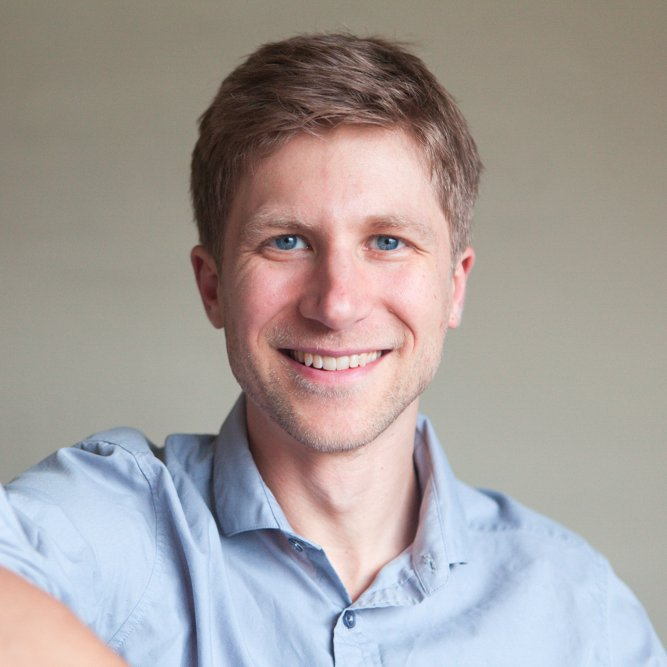
\includegraphics[height=2cm]{collaborators/ryan}
  			\caption*{Ryan Giordano \\ MIT}
  		\end{subfigure}
  		\begin{subfigure}{.4\textwidth}
  			\centering
  			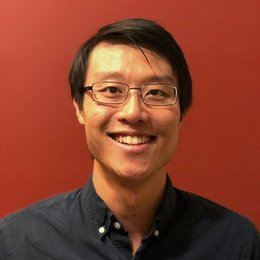
\includegraphics[height=2cm]{collaborators/bryan}
        \captionsetup{justification=centering}
  			\caption*{Runjing (Bryan) Liu \\ UC Berkeley}
  		\end{subfigure}\\%
  		\vspace{0.11in}
      \begin{subfigure}{.4\textwidth}
  			\centering
  			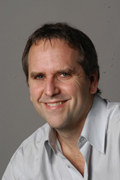
\includegraphics[height=2cm]{collaborators/mike}
  			\caption*{Michael I.\ Jordan \\ UC Berkeley}
  		\end{subfigure}%
  		\begin{subfigure}{.4\textwidth}
  			\centering
  			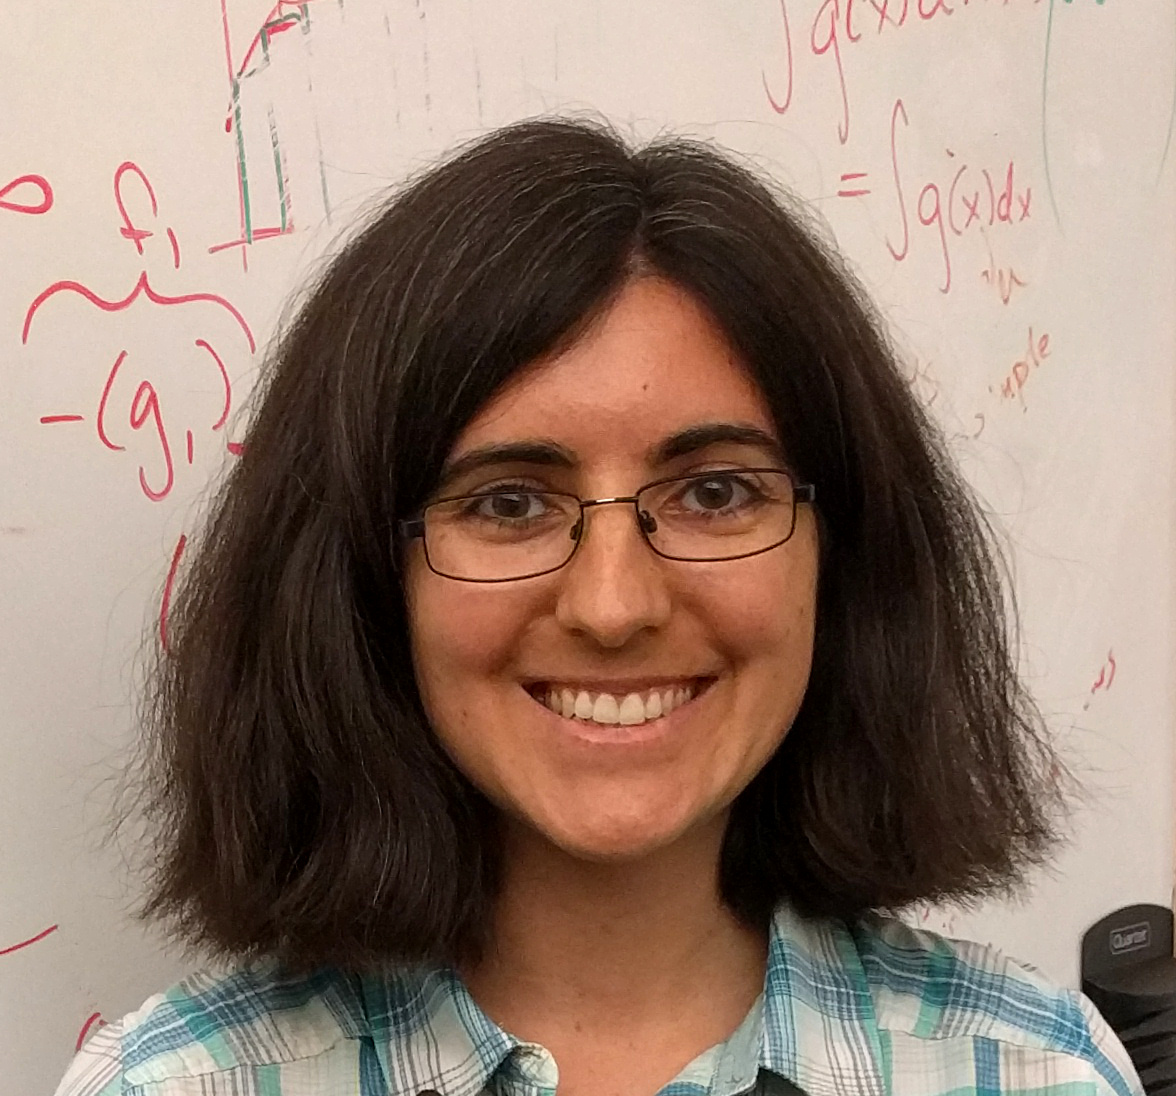
\includegraphics[height=2cm]{collaborators/tamara}
  			\caption*{Tamara Broderick \\ MIT}
  		\end{subfigure}\\
  	\end{figure}


\end{frame}


\begin{frame}{Motivating Example}

Inferring population structure from genomic sequences.
\begin{itemize}
  \item[--] Genetic data from Taita thrush, an endangered bird species native to Kenya
  \citep{galbusera:2000:thrush}
  %{\color{blue} \href{https://web.stanford.edu/group/pritchardlab/publications/pdfs/Pritch%ardEtAl00.pdf}{(Pritchard et al. 2000)}}
  \item[--] Microsatellites sequences of 155 individuals at 7 loci.
\end{itemize}


\begin{figure}[!h]
\centering
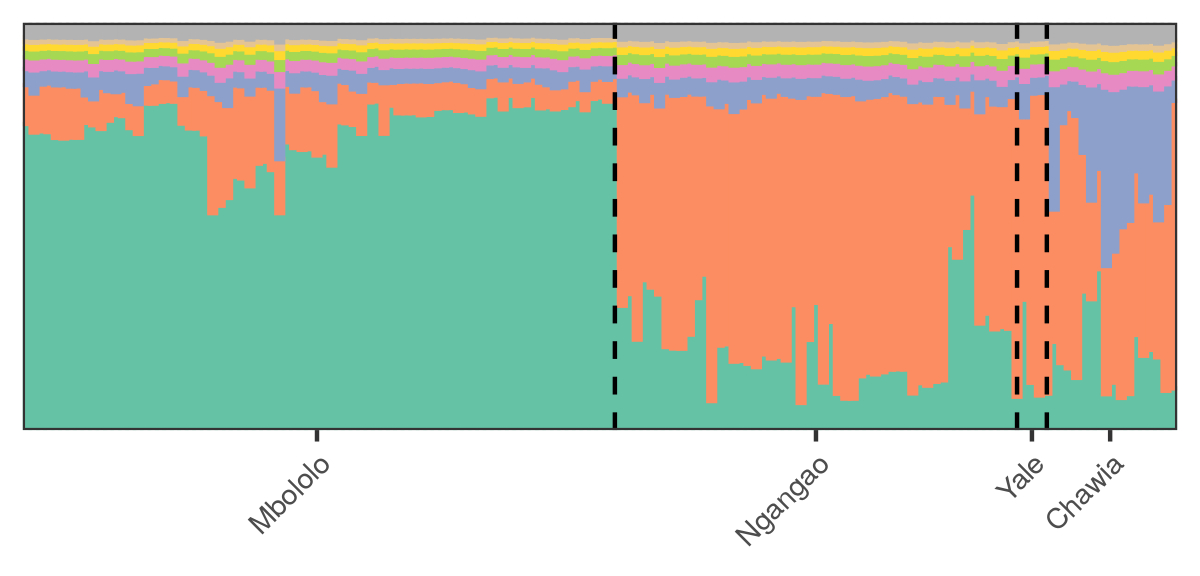
\includegraphics[width = 0.9\textwidth]{./figure/structure_init-1.png}
\end{figure}

\end{frame}

\begin{frame}{Motivating Example}

\begin{figure}[ht!]
\centering
\only<1-2>{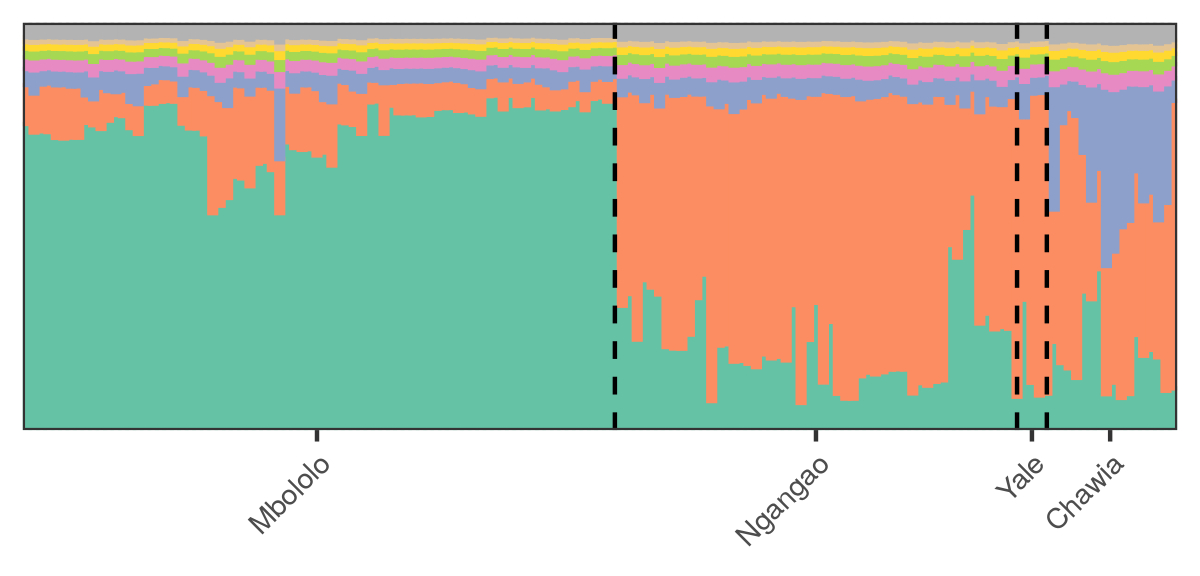
\includegraphics[width = 0.9\textwidth]{./figure/structure_init-1.png}}
\only<3>{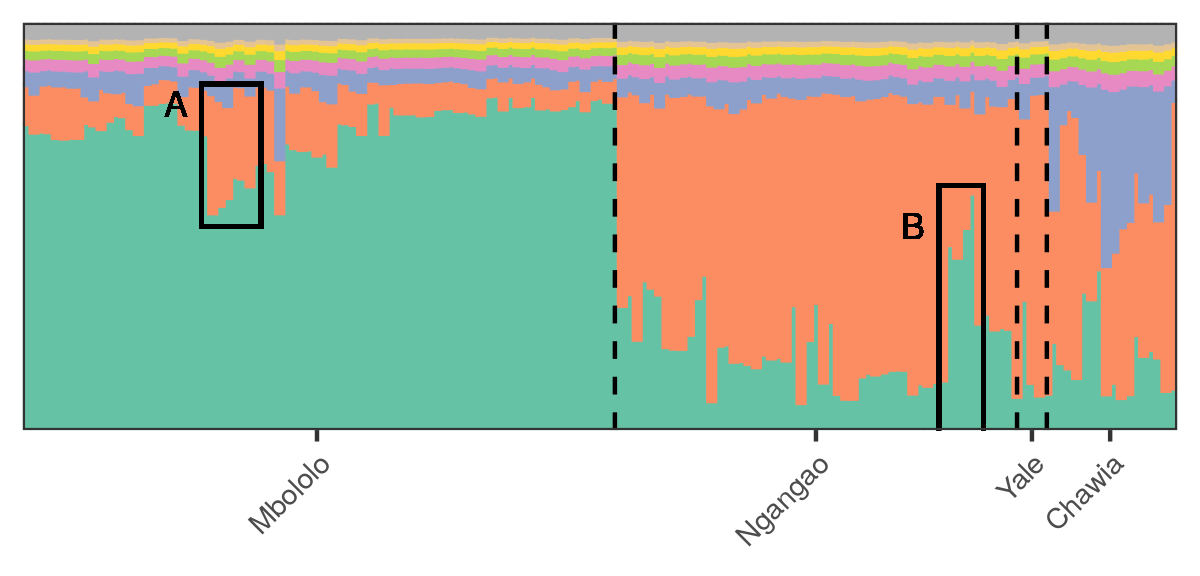
\includegraphics[width = 0.9\textwidth]{./figure/structure_migration-1.png}}
\end{figure}
\vspace{-1em}

%%%%%%%%%%%%%
% how many latent populations?
%%%%%%%%%%%%%
\only<1>{
%\textbf{How many latent populations (clusters) are present in the data set?}

- Three primary populations
{\large
\textcolor{pop1}{$\blacksquare$}
\textcolor{pop2}{$\blacksquare$}
\textcolor{pop3}{$\blacksquare$}
}.

- Many small, rare populations
{\large 
\textcolor{pop4}{$\blacksquare$}
\textcolor{pop5}{$\blacksquare$}
\textcolor{pop6}{$\blacksquare$}
\textcolor{pop7}{$\blacksquare$}
\textcolor{pop8}{$\blacksquare$}
}. 

{\bf Question: How many distinct populations (clusters) are there...}
\vspace{-0.5em}
\begin{itemize}
    \item ...in this dataset?
    \item ...with more than $N$ loci?
    \item ...in a future dataset of the same size?
\end{itemize}
\vspace{3.5em}
}



%%%%%%%%%%%%%
% coclustering
%%%%%%%%%%%%%
\only<2-3>{
Individuals are generally clustered by geographic locations:
\begin{minipage}{0.3\textwidth}
 Mbololo $\approx$ {\large \textcolor{pop1}{$\blacksquare$}}
\end{minipage}
\begin{minipage}{0.3\textwidth}
 Ngangao $\approx$ {\large \textcolor{pop2}{$\blacksquare$}}
\end{minipage}
\begin{minipage}{0.35\textwidth}
Chawia $\approx$
    {\large 
    \textcolor{pop1}{$\blacksquare$} + 
    \textcolor{pop2}{$\blacksquare$} + 
    \textcolor{pop3}{$\blacksquare$}}
\end{minipage}

\textbf{Question: Which individuals cluster together?}

Exceptions to the clustering give evidence of historical migrations.
}

\only<2> {
% so that the figure aligns across the \only ....
% is there a better way to do this?
\vspace{2em}
}
\only<3>{
For example, the groups of individuals in A and B suggest migration
between the Mbololo and Ngangao locations. 
}
\end{frame}



\begin{frame}{Motivating Example}
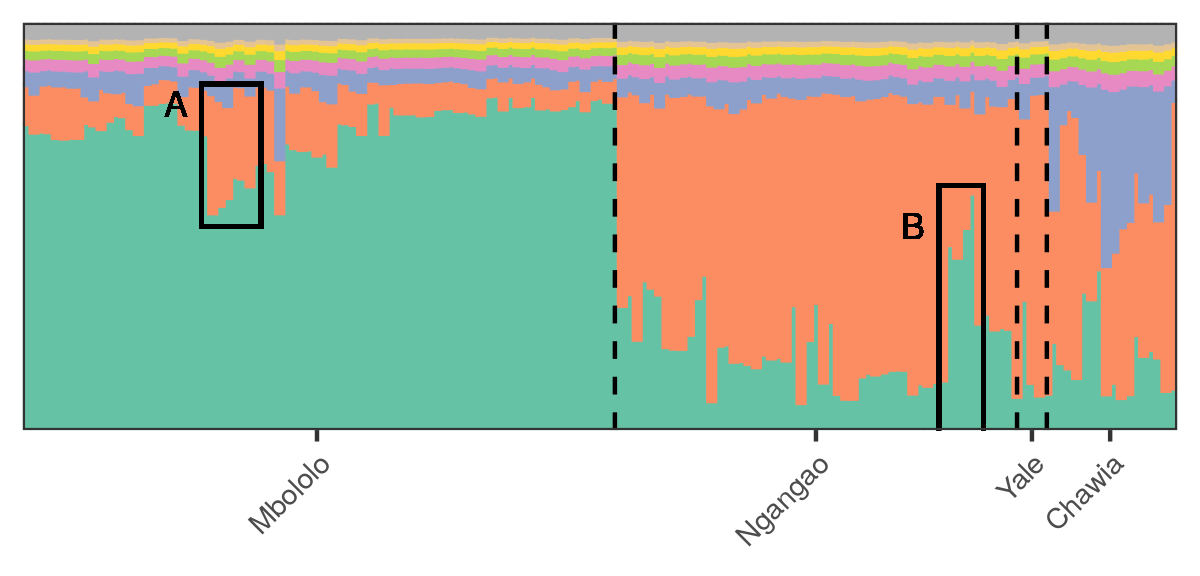
\includegraphics[width = 0.9\textwidth]{./figure/structure_migration-1.png}

How many distinct clusters are there?
%
Which individuals cluster together?

A \textbf{discrete Bayesian nonparametric (BNP)} model makes these questions 
amenable to Bayesian inference...

...but the answer may depend on the \textbf{prior you choose.}

\end{frame}


\begin{frame}{Motivating Example}

\begin{figure}[!h]
\centering
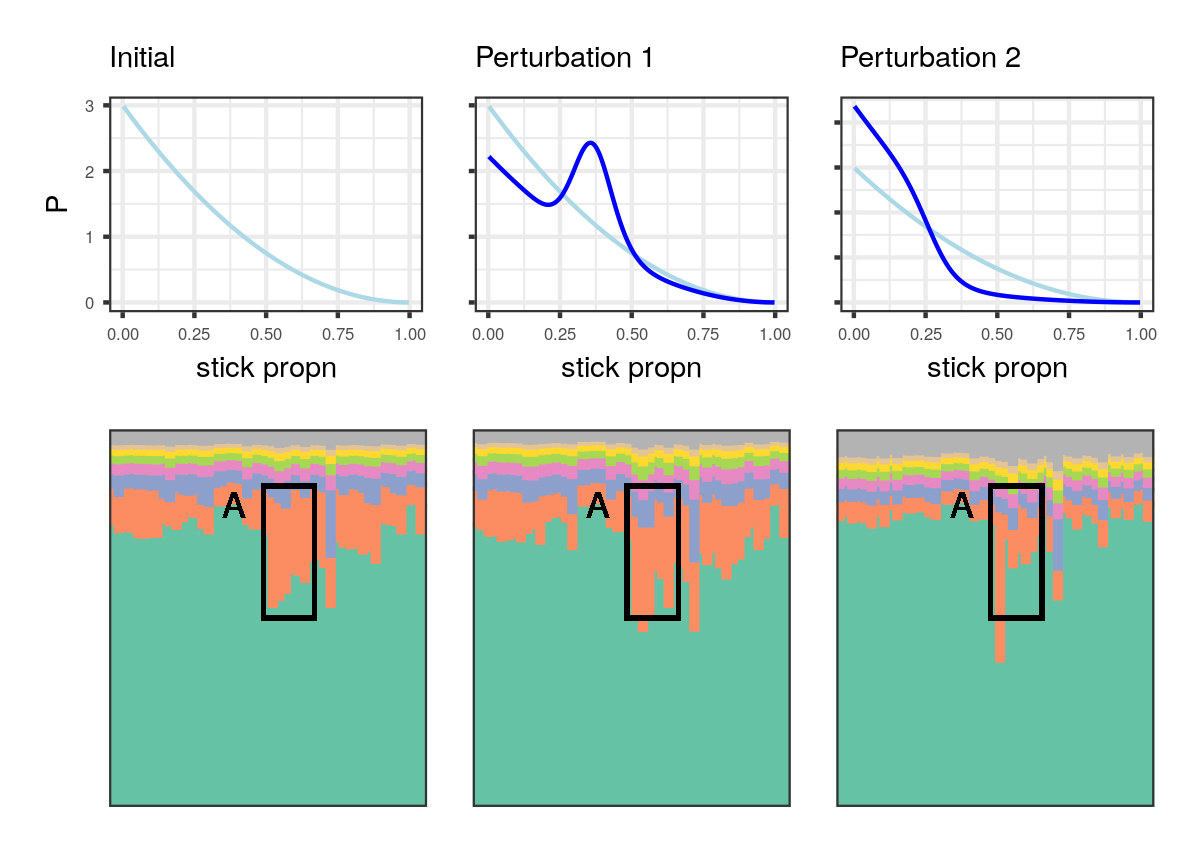
\includegraphics[width = \textwidth]{./figure/mbololo_motivating_ex-1.png}
\end{figure}

\end{frame}



\begin{frame}{Research Problem}

A discrete Bayesian nonparametric (BNP) model makes scientific
questions amenable to Bayesian inference.

\pause

We approximate the exact posterior using variational Bayes (VB).

\pause

\textbf{Question}: How sensitive is the VB approximation, and the resulting
inferences, to BNP model choices?

\pause

\textbf{Problem}: Re-running VB for multiple model choices is expensive.

\pause

\textbf{We propose}: A linear approximation to efficiently
estimate BNP sensitivity from a single run of VB.  The linear approximation
can both:
\begin{itemize}
    \item Provide approximate sensitivity with no refitting, or
    \item Guide the choice of priors for refitting.
\end{itemize}

\end{frame}



\begin{frame}{Outline}
\begin{itemize}
\item The BNP model
\vspace{0.1in}

\item The variational approximation
\vspace{0.1in}

\item Hyperparameter sensitivity
\vspace{0.1in}

\item Functional sensitivity and influence functions
\vspace{0.1in}

\item Results on population genetics modeling of the Taita thrush
\vspace{0.1in}

\end{itemize}
\end{frame}


\begin{frame}{The BNP Model \citep{sethuraman:1994:constructivedp}}
A {\bf Dirichlet process prior} allows for an infinite number of components.
\vspace{-0.2em}
\begin{figure}[!h]
\centering
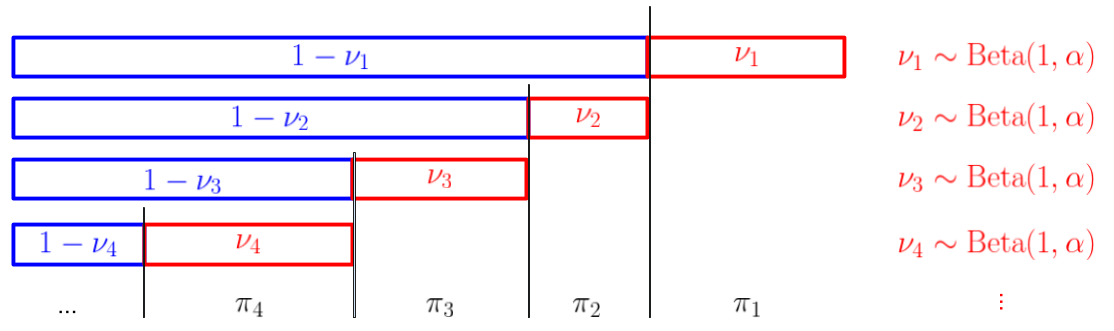
\includegraphics[width = 0.95\textwidth]{./static_figures/DP_stick_breaking.png}
\caption{A schematic of the Dirichlet process prior}
\end{figure}
\vspace{-0.2in}

While there are an infinite number of {\bf components}, there are a finite number of {\bf clusters} in a given dataset. 
%\pause 

Posterior quantities depend on the BNP prior, which is defined 
by the density of the stick-breaking process $\nuk \sim \p(\nuk)$.


% \begin{enumerate}[(1)]
% \item How many clusters are in the {\itshape current} dataset?

% %\pause
% \item How many clusters would we expect to see in a {\itshape new} dataset?
% \item Which observations in the current dataset cluster together?

% \end{enumerate}

% \pause

% These quantities depend on the choice of stick-breaking prior.

%\pause

\vspace{1em}

\begin{mdframed}[style=MyFrame]
\begin{center}
{\bf If $\nuk \sim \betadist{1, \alpha}$ what should $\alpha$ be?\\}
{\bf Why should $\p(\nuk)$ even be in the Beta family?}
\end{center}
\end{mdframed}

\end{frame}


\begin{frame}{The Variational Approximation}

Let $\theta$ be unknown parameters and $y$ the data.

We posit a class of mean-field distributions parameterized by a real vector $\eta$.

We solve
\begin{align*}
  \eta^* = \argmin_{\eta} KL\left(
      q(\theta \vert \eta )\big\| p(\theta | y)
      \right)
\end{align*}

\only<1>{
\begin{figure}[!h]
\centering
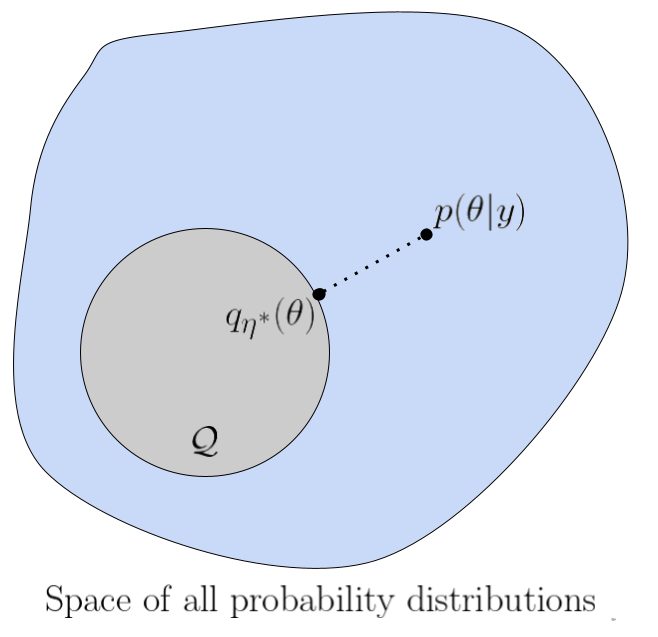
\includegraphics[width = 0.4\textwidth]{./figures/vi_schematic2.png}
\end{figure}
}

\only<2->{
Note that

\begin{itemize}
\item The optimal variational parameters $\eta^*$ depend on the prior through optimizing the KL objective.

\pause

\item The approximate posterior quantities are then functions of $\eta^*$, e.g.\
\begin{align*}
\eta^* \mapsto
\Expect_{q_{\eta^*}} \left[ \#\text{clusters} \right]
\quad \text{ or } \quad
\eta^* \mapsto
\Expect_{q_{\eta^*}}
\left[\#\{\substack{\text{clusters in}\\\text{new dataset}}\} \right].
\end{align*}

\end{itemize}
}

\only<3>{
\begin{mdframed}[style=MyFrame]
\begin{center}
{\bf How do these approximate posterior quantities depend on the DP prior?}
\end{center}
\end{mdframed}
}
\end{frame}


\begin{frame}{Hyperparameter Sensitivity}

Let $\t$ be some real-valued hyperparameter for the stick-breaking density.
%(For example, $\t$ could be $\alpha$, or parameterize a functional shape).  
\pause

Write $\etaopt(\t) := \argmin_{\eta} \KL{\eta, \t} = \argmin_{\eta} \KL{\q(\zeta \vert \eta) || \p(\zeta \vert \x, \t)}$.
\pause

{\bf Problem:} Evaluating $\etaopt(\t)$ requires solving a new optimization problem.
\pause

%\pause

{\bf We propose: } Approximate $\etaopt(\t)$ with a first-order
Taylor expansion:

\begin{align*}
  \etaopt(\t)  &\approx  
  %\etalin(\t) := 
  \etaopt(0) + \fracat{d \etaopt(\t)}{d \t}{\t=0} \t. 
\end{align*}
%
\pause
%
\vspace{-0.5em}
\begin{itemize}
\item<5-> We need only use a linear approximation for the map $\t \mapsto \etaopt(\t)$. We can retain nonlinearities in the map 
$\etaopt \mapsto \expect{\q(\zeta \vert \etaopt)}{\#\text{clusters}}
$, etc.
\vspace{0.5em}
\item<6-> This is ``Bayesian local robustness'' for VB \citep[cf.][]{gustafson:1996:local}
\vspace{0.5em}
\item<7-> The derivative can be evaluated using the implicit function theorem
and modern
{\color{blue} \href{https://jax.readthedocs.io/en/latest/}{automatic differentiation}}.
\end{itemize}
\end{frame}







\begin{frame}{Computing the Derivative \citep{giordano:2018:covariances}}

\textbf{Theorem 1.} (The derivative $d\etaopt(\t) / d\t$.)  

\onslide<2-> {
Define $\etaopt = \etaopt(0)$, $\hessopt := \fracat{\partial^2 \KL{\eta}}
                {\partial \eta \partial \eta^T}
                {\etaopt}$ and 
$\lqgrad{\nu \vert \etaopt} :=
    \fracat{\log \q(\nu \vert \etaopt)}{\partial \eta}{\etaopt}$.
}

\onslide<3->Assume:
\begin{itemize}
    \item<3-> The Hessian at the optimum, $\hessopt$, is non-singular. %\pause
    \item<4-> The optimal VB parameters, $\etaopt$, are interior. %\pause
    \item<5-> We can exchange limits and $\q$ expectations as needed in a 
        neighborhood of $\etaopt$ and $\t=0$.  %\pause
    \begin{itemize}
        %\item Dominated convergence theorem on a laundry list of functions.
        \item This imposes some regularity conditions on the prior $\p(\nu \vert \t)$.
    \end{itemize}
\end{itemize}

\onslide<6->{
Then the map $\t \mapsto \etaopt(\t)$ is continuously
differentiable at $\t=0$ with
%
\begin{align*}
%
\fracat{d \etaopt(\t)}{d \t}{0} ={}&
    - \hessopt^{-1}
    \expect{\q_{\etaopt}}{
        \lqgrad{\nu \vert \etaopt}
        \fracat{\partial \log \p(\nu \vert \t)}{\partial \t}{\t=0}
    }.
%
\end{align*} \hfill $\square$
}

\onslide<7->{
{\bf Note:} The computation of $\hessopt^{-1}$ is the computationally 
difficult part.  For our BNP problem, $\hessopt$ is sparse.
}

\end{frame}

\begin{frame}{A Simple Example: Iris Data}

We fit a Gaussian mixture model with a DP prior to
the iris data.

\begin{figure}[!h]
  \centering
  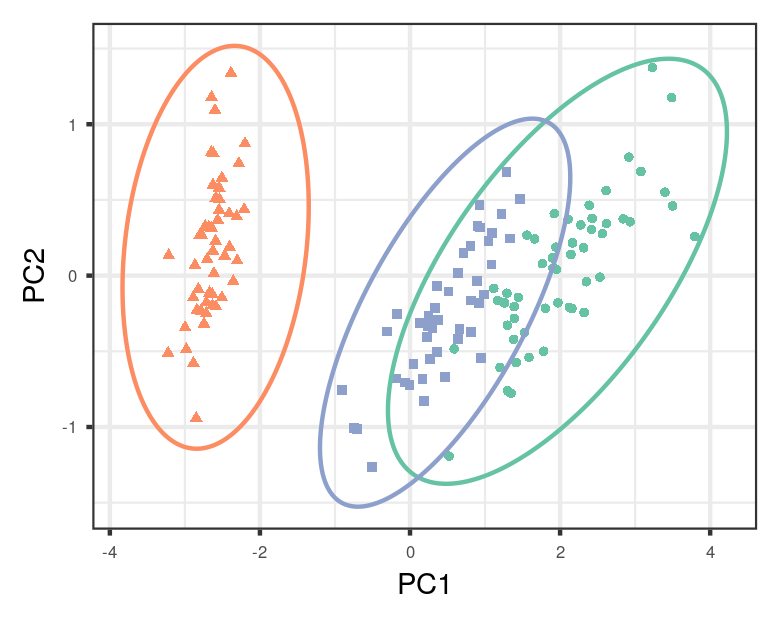
\includegraphics[width = 0.6\textwidth]{./figure/iris_init-1.png}
  \caption*{The iris data in principal component space and GMM fit at $\alpha = 6$.}
\end{figure}

\end{frame}

\begin{frame}{Iris Data: Parametric Sensitivity}

\begin{figure}[!h]
  \only<1>{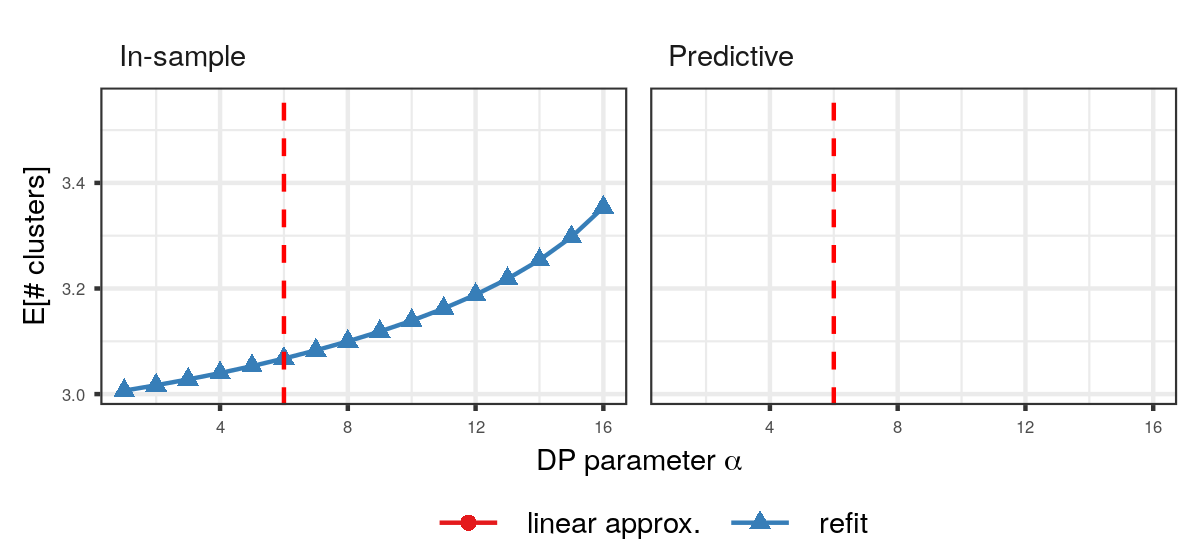
\includegraphics[width = \textwidth]{./figure/iris_alphasens_refit-1.png}}%
  \only<2>{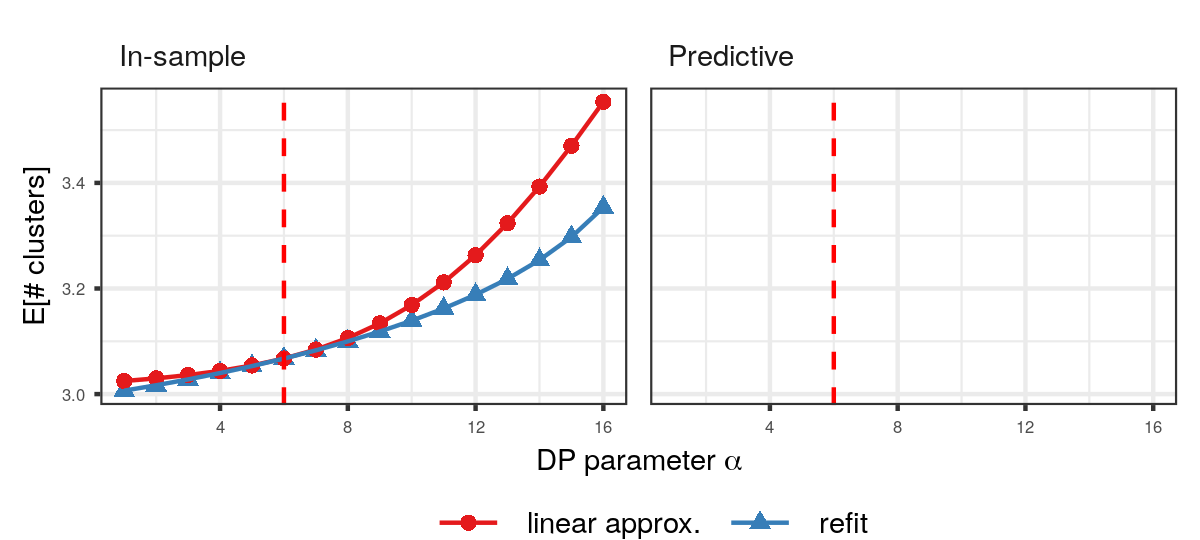
\includegraphics[width = \textwidth]{./figure/iris_alphasens_insample-1.png}}%
  \only<3>{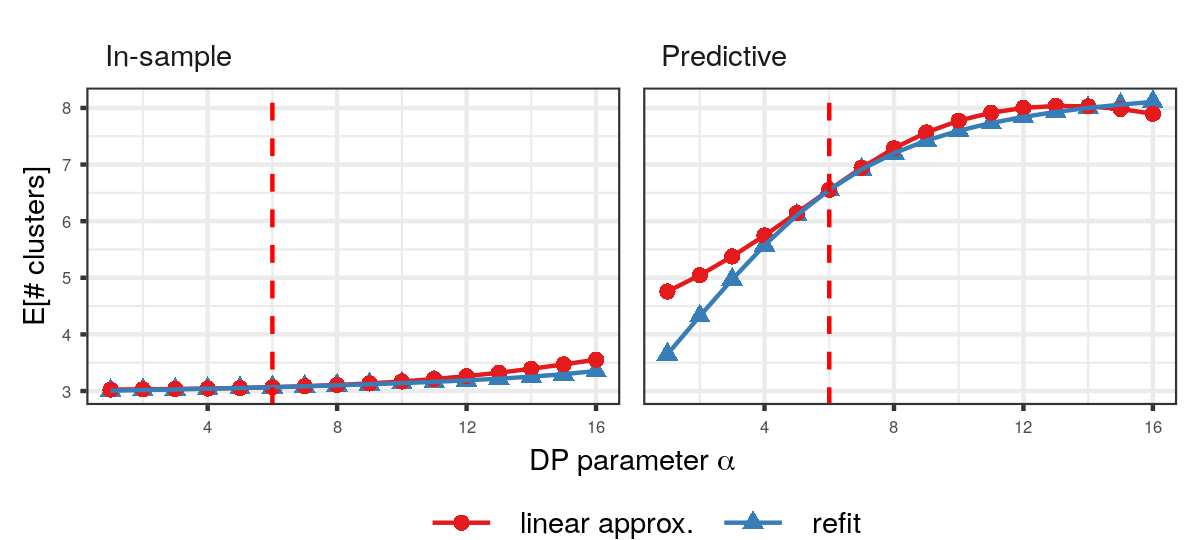
\includegraphics[width = \textwidth]{./figure/iris_alphasens_all-1.png}}
  \caption*{The expected number of posterior clusters in the iris data as $\alpha$ varies.}
\end{figure}

\end{frame}


\begin{frame}{Functional Sensitivity  \citep{gustafson:1996:local}}

\vspace{1em}

\begin{mdframed}[style=MyFrame]
\begin{center}
{\bf What about stick-breaking priors not in the Beta family?}
\end{center}
\end{mdframed}
\pause
Let $\p_0(\nu)$ be the stick-breaking prior used to compute $\etaopt$.
Suppose we wish to replace $\p_0(\nu)$ with another density, $\p_1(\nu)$. 

\pause
Define the ``perturbed'' prior as:
\begin{align*}
\p(\nu \vert \phi) \propto
\pbase(\nu)\exp(\phi(\nu))
\quad\textrm{with}\quad
\phi(\nu) = \log \p_1(\nu) - \log \p_0(\nu)
\end{align*}

\pause 

Then $\t \mapsto \p(\nu \vert \t \phi)$ 
parameterizes a path from $\pbase$ to $\palt$ for $\t \in [0,1]$.

\pause

\begin{figure}[!h]
\centering
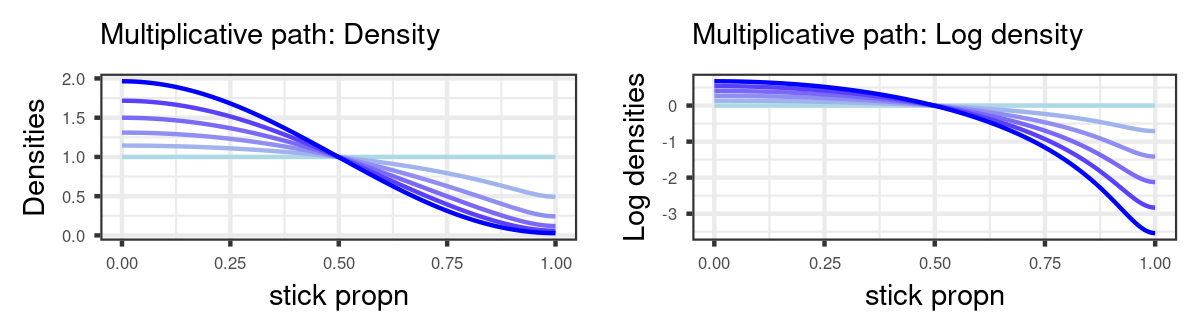
\includegraphics[width = 1.0\textwidth]{./figure/mult_path-1.png}
\setlength{\textfloatsep}{-10pt}
\end{figure}

\end{frame}





\begin{frame}{Functional Sensitivity  \citep{gustafson:1996:local}}

For any particular $\phi$, we can try to apply Theorem 1
to $\t \mapsto \p(\nu \vert \t \phi)$.  
          
\onslide<2->{
But it would be nice to safely search the space of functions $\phi$.
}

\onslide<3-> {
{\bf Questions:}
\begin{itemize}
    \item Can we specify a general condition on $\phi$ for
          Theorem 1 to apply?
    \item<4-> Is the derivative a good linear approximation for all
          such functions?
\end{itemize}
}

\begin{figure}[!h]
\centering
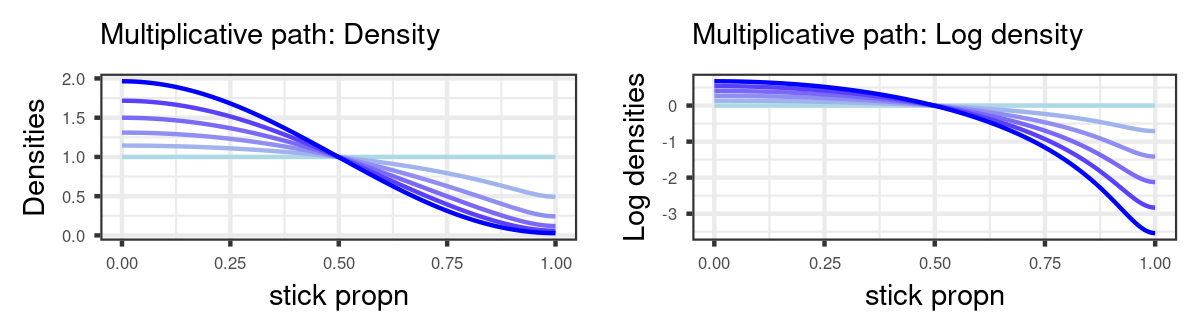
\includegraphics[width = 1.0\textwidth]{./figure/mult_path-1.png}
\setlength{\textfloatsep}{-10pt}
\end{figure}


\end{frame}









\begin{frame}{Functional Sensitivity: Differentiability}

% Let $\lp{\infty}$ denote the vector space of pointwise bounded functions
% measurable with respect to a measure dominating $\q(\nu \vert \eta)$ and $\pbase(\nu)$.
Let $\lp{\infty}$ denote the vector space of bounded, Lebesgue-measurable functions
with norm $\norminf{\phi} := \esssup_\nu \abs{\phi(\nu)}$.

\onslide<2->{
\textbf{Proposition.}

If $\phi \in \lp{\infty}$, then $\p(\nu \vert \phi)$ is a valid density
(positive and normalizable).
}

\onslide<3->{
\textbf{Theorem 2.}  (Validity of the derivative in $\lp{\infty}$.)
}

\onslide<4->{
If $\phi \in \lp{\infty}$, then the map $\t \mapsto \p(\nu \vert \t\phi)$
satisfies the conditions of Theorem 1, so $\t \mapsto \etaopt(\t \phi)$
is continuously differentiable.
}

\onslide<5->{
Further, the derivatives provides a uniformly
good linear approximation in an $\norminf{\cdot}$-neighborhood of the zero function.
%
In other words, the map $\phi \mapsto \etaopt(\phi)$ from
$\lp{\infty} \mapsto \mathbb{R}^D$ is {\em Fr{\'e}chet differentiable} at 
zero. \hfill $\square$
}

\onslide<6->{
{\bf Note:} Arguably, Fr{\'e}chet differentiability is a
minimal requirement for using the linear
approximation to safely search the space of functions.
}

\end{frame}





\begin{frame}{Functional Sensitivity: Influence Functions}

\textbf{Corollary of Theorem 2.} (Influence functions.)

Take a continuously differentiable quantity of
interest $g(\eta)$, e.g.
\begin{align*}
\g_{\textrm{cl}}(\eta) = \expect{\q_{\eta}} {\#\text{clusters}}
\end{align*}

\pause 
Let $S_g(\phi)$ be the \textit{local sensitivity} of $g$ in the direction $\phi$:
\begin{align*}
S_g(\phi) := \fracat{d g(\etaopt(\t \phi)) }{d\t}{\t=0}. 
\end{align*}

\pause

If $\norminf{\phi} < \infty$, the local sensitivity can be expressed as
an inner product between
an \textit{influence function} $\infl$ and the functional perturbation $\phi$:
\begin{align*}
S_g(\phi)   &=
    - \fracat{d g(\eta)}{d \eta^T}{\etaopt}
    \hessopt^{-1}
    \expect{\q_{\etaopt}}{
        \lqgrad{\nu \vert \etaopt}
        \phi(\nu)
    }
\\&=
\int \Psi(\nu) \phi(\nu) \;d\nu.
\end{align*}

\end{frame}








\begin{frame}{Iris Data: Influence Functions}
  \begin{figure}[!h]
    \centering
    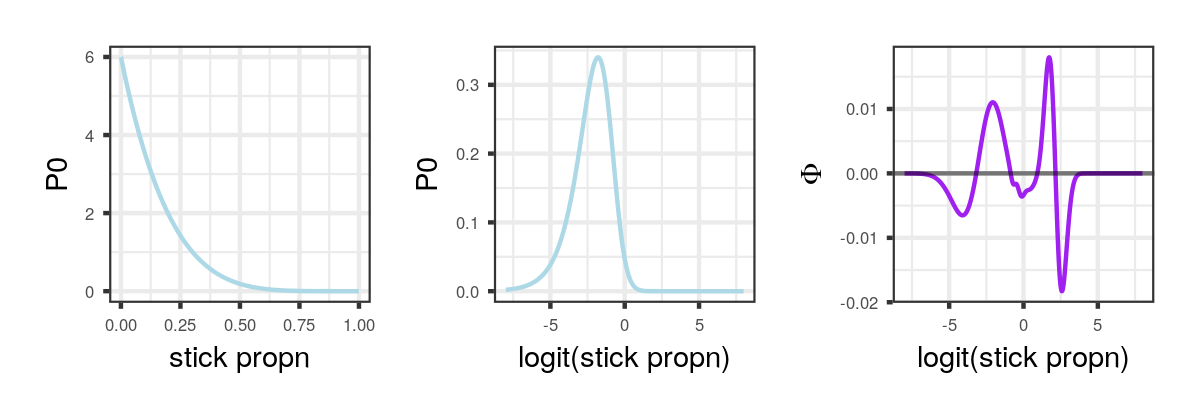
\includegraphics[width = \textwidth]{./figure/iris_infl-1.png}
    \caption*{The influence function for the number of clusters, $g_{\textrm{cl}}$.}
\end{figure}
\end{frame}

\begin{frame}{Iris Data: Functional Perturbations}
\begin{figure}[!h]
    \centering
    \only<1>{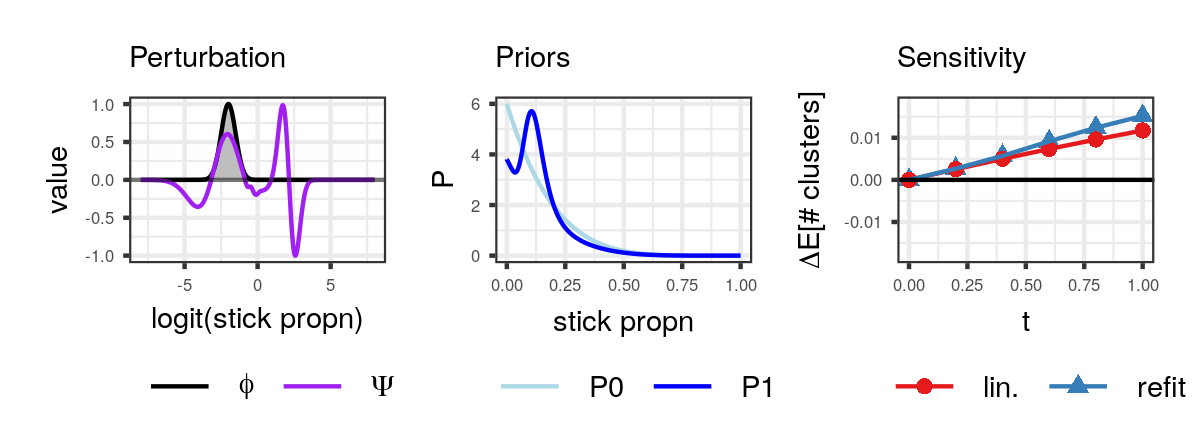
\includegraphics[width = \textwidth]{./figure/iris_fpertex-1.png}}
    \only<2>{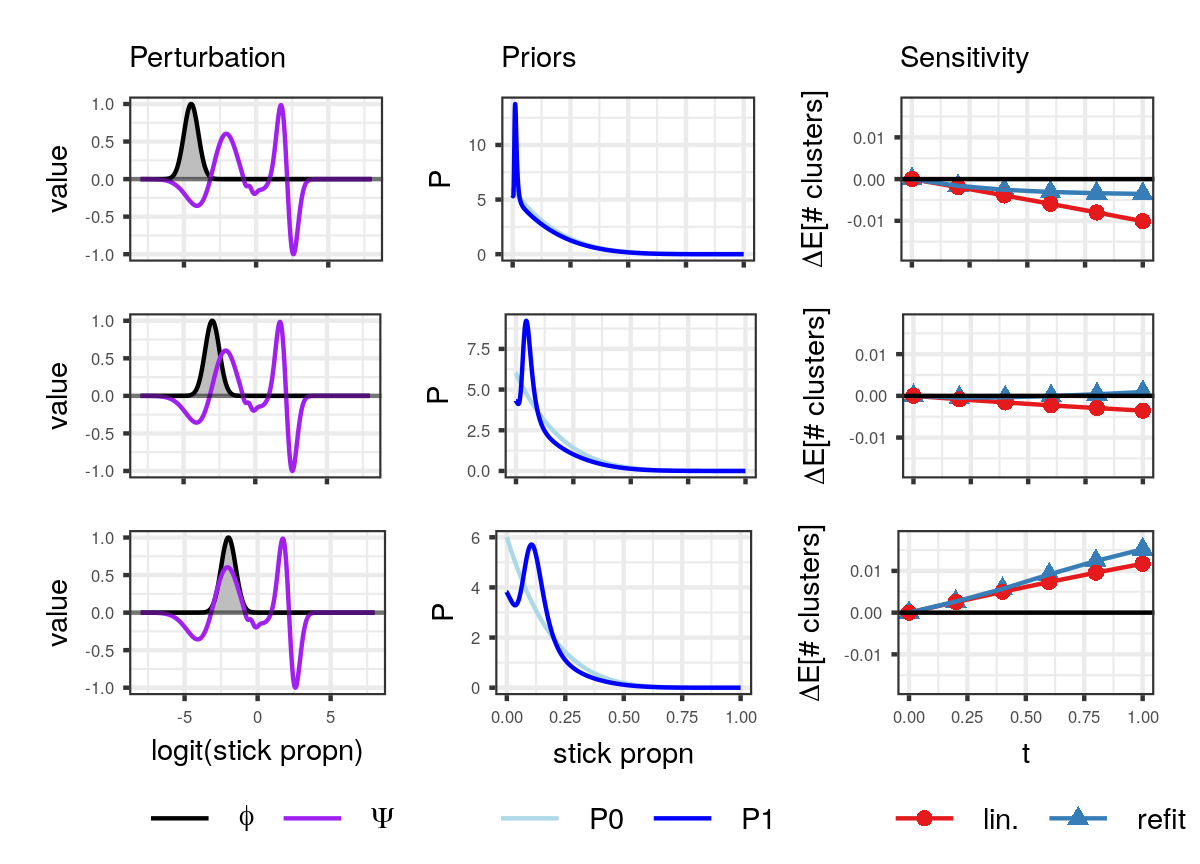
\includegraphics[width = \textwidth]{./figure/iris_fpertall-1.png}}
\end{figure}
\end{frame}






\begin{frame}{Functional Perturbations: Worst Case \citep{gustafson:1996:local}}

Which perturbation $\phi$ maximizes the sensitivity $S_g(\phi)$?

\pause
That is, can we find the {\bf worst-case} $\phi$ in the L-infinity ball of radius $\delta$,
%
\begin{align*}
  B_\delta := \{\phi : \|\phi\|_\infty < \delta\}?
\end{align*}

\vspace{-1em}

\pause
\begin{figure}[!h]
\centering
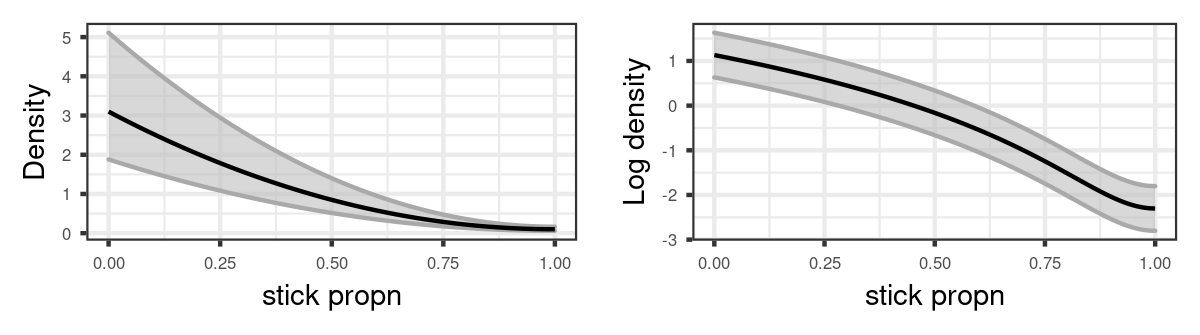
\includegraphics[width = 1.0\textwidth]{./figure/func_ball-1.png}
\setlength{\textfloatsep}{-10pt}
\end{figure}

\vspace{-2em}

\pause
Using the influence function and H{\"o}lder's inequality,
%
\begin{align*}
%
\sup_{\phi \in \ball_\delta} S_g(\phi) ={}&
\sup_{\phi \in \ball_\delta} \int \infl(\nu)\phi(\nu) d\nu
= \delta \int \abs{\infl(\nu)} d\nu, \textrm{ achieved at} \\
\phi^*(\nu) ={}& \delta \; \mathrm{sign}(\infl(\nu)).
%
\end{align*}
%
%achieved at $\phi^*(\nu) = \delta \; \mathrm{sign}(\infl(\nu))$.
%
\end{frame}






\begin{frame}{Iris Data: Worst-Case Perturbation}
  \begin{figure}[!h]
    \centering
    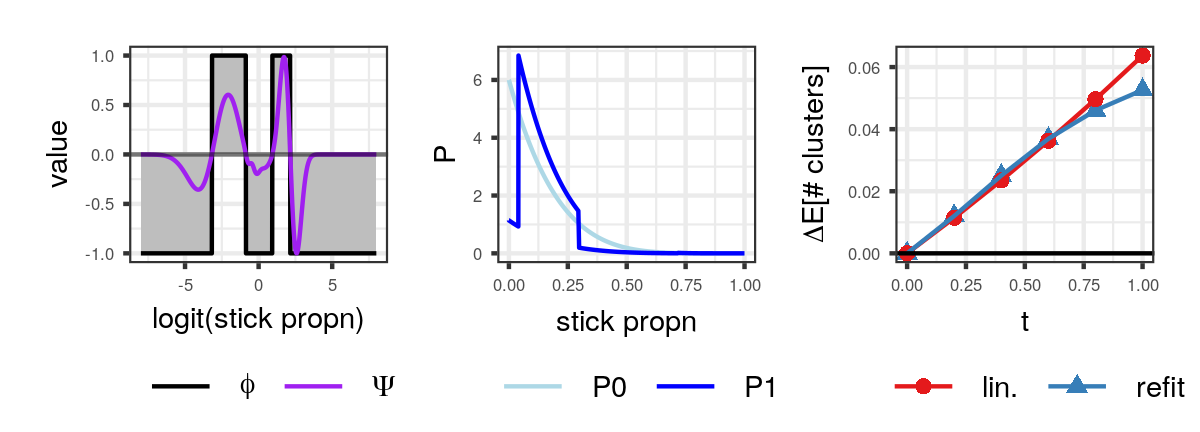
\includegraphics[width = \textwidth]{./figure/iris_worstcase-1.png}
\end{figure}

\pause

The worst-case prior may look unreasonable.  

But if the worst-case sensitivity is small, it is evidence of robustness.
\end{frame}


\begin{frame}{Functional sensitivity: other paths \citep{gustafson:1996:local}}

For $\p(\nuk \vert \phi)$, we used a multiplicative perturbation.

\vspace{1em}

\begin{mdframed}[style=MyFrame]
\begin{center}
{\bf Could we have used other paths through function space? }
\end{center}
\end{mdframed}

\pause

%Recall that we used $\p(\nuk \vert \phi) \propto \pbase(\nuk)\exp(\phi(\nuk))$.
Consider, for example, ``mixture distributions'':
%
\begin{align*}
\p(\nu \vert \phi_{mix}) \propto{}
\pbase(\nu) + \phi_{mix}(\nu)
\quad\textrm{and}\quad
\phi_{mix}(\nu) = \palt(\nu) - \pbase(\nu)
\end{align*}

\vspace{-0.5em}
Then $\t\mapsto \p(\nu \vert t\phi_{mix})$ also parameterizes a path from
$\pbase$ to $\palt$.

\pause

\vspace{-0.5em}
\begin{figure}[!h]
\centering
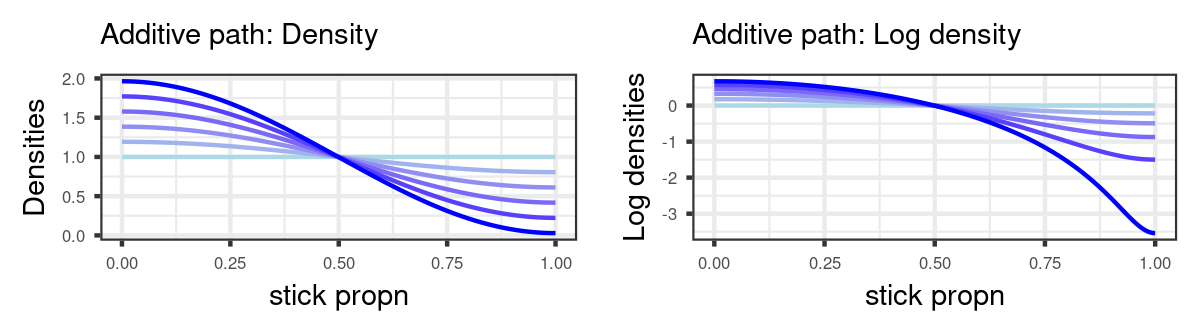
\includegraphics[width = 0.8\paperwidth]{./figure/lin_path-1.png}
%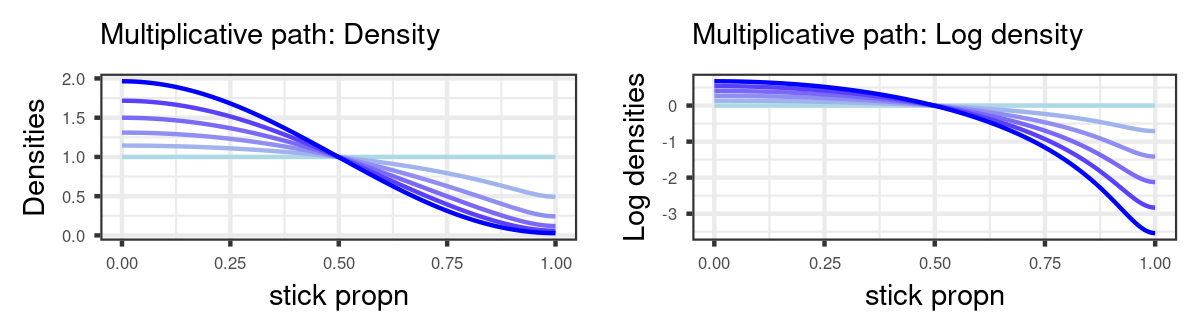
\includegraphics[width = 0.7\paperwidth]{./figure/mult_path-1.png}
\end{figure}
%
%\vspace{-1.5em}

\pause

{\centering
{\bf Question:} Is there anything wrong with using $\phi_{mix}$ with our VB approximation?
}
\end{frame}




\begin{frame}{Functional Sensitivity: Other Paths}

% \textbf{Proposition (c.f. \citet{gustafson:1996:local})}

% If $\norm{\phi_{mix}}_1 := \int_0^1 \abs{\phi_{mix}(\nu)} d\nu$ is small, then
% $\p(\nu \vert \phi_{mix})$ can be normalized.

% If $\p(\nu \vert \phi_{mix})$ can be normalized, then $\norm{\phi_{mix}}_1 < \infty$.

% \pause

% $\Rightarrow$ $\norm{\cdot}_1$ is the sensible norm for mixture perturbations.

\pause

\textbf{Theorem 3.} (Differentiability of other paths.)

\pause 

Let
$S_{mix} := \{\phi_{mix}: \phi_{mix} =
 \palt - \pbase \textrm{ for some density }
 \palt \ll \pbase \}$.

\pause 

For any $\phi_{mix} \in S_{mix}$, the conditions of 
Theorem 1 are satisfied under some additional mild integrability
assumptions on $\q_\eta$.  So the map $\t \mapsto \etaopt(\t \phi_{mix})$
is continuously differentiable.

\pause

But normalizability of $\p(\nu \vert \phi_{mix})$ is determined by
$\norm{\phi_{mix}}_1$, and the error of the derivative is
arbitrarily large in any $\norm{\cdot}_1$-neighborhood of the zero function.

\pause

$\Rightarrow$ No extension
of $S_{mix}$ to $\lp{1}$ of the map $\phi_{mix} \mapsto \etaopt(\phi_{mix})$ 
can be Fr{\'e}chet differentiable. 

% ...and the map
% $\phi_{mix} \mapsto \KL{\etaopt, \phi_{mix}}$ is discontinuous
% in $\norm{\cdot}_1$ on $S_{mix}$.

% Fr{\'e}chet differentiability implies
% continuity.  Consequently, no extension
% of $S_{mix}$ to $\lp{1}$ of the map $\phi_{mix} \mapsto \etaopt(\phi_{mix})$ 
% can be Fr{\'e}chet differentiable.  

\hfill $\square$

\pause

\textbf{Note:}
An analogous result holds for all $\lp{p}$ spaces with $p < \infty$.

\end{frame}






\begin{frame}{Functional Sensitivity: Other Paths}

{\bf What went wrong with the mixture distribution?}

\begin{minipage}{0.49\textwidth}
\onslide<2->{
These red and blue densities are
\begin{itemize}
    \item Distant in KL and $\norminf{\cdot}$, but
    \item Close in $\norm{\cdot}_p$ when $p < \infty$.
\end{itemize}
}

\onslide<3->{
\vspace{1em}
A parameterization + prior normalizability dictates a norm.
}

\onslide<4->{
\vspace{1em}
For differentiability of $\etaopt$, the norm's topology must match that of KL.
}

\onslide<5->{
\vspace{1em}
$\Rightarrow$ {\bf We consider only multiplicative perturbations for VB.}
}

%
\end{minipage}
%
% Figure minipage
\begin{minipage}{0.49\textwidth}
\onslide<2->{
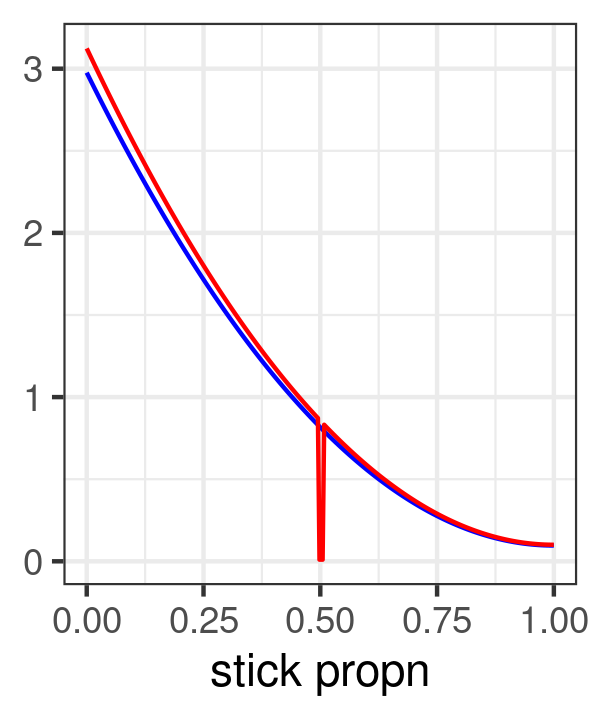
\includegraphics[width=1.0\linewidth,height=1.176\linewidth]{figure/func_dist-1} 
}
\end{minipage}

\end{frame}



\begin{frame}{Results on fastSTRUCTURE \citep{raj:2014:faststructure}}

We adapt fastSTRUCTURE
% {\color{blue} \href{https://web.stanford.edu/group/pritchardlab/publications/pdfs/PritchardEtAl00.pdf}{(Pritchard et al. 2000};
% \href{https://www.genetics.org/content/197/2/573}{Raj et al. 2014)}
% },
a Bayesian model for population genetics, to include a BNP prior.


We study genetic data from the Taita thrush, an endangered bird species.
The data consists of microsatellites sequences of 155 individuals at 7 loci.

\begin{figure}[!h]
\centering
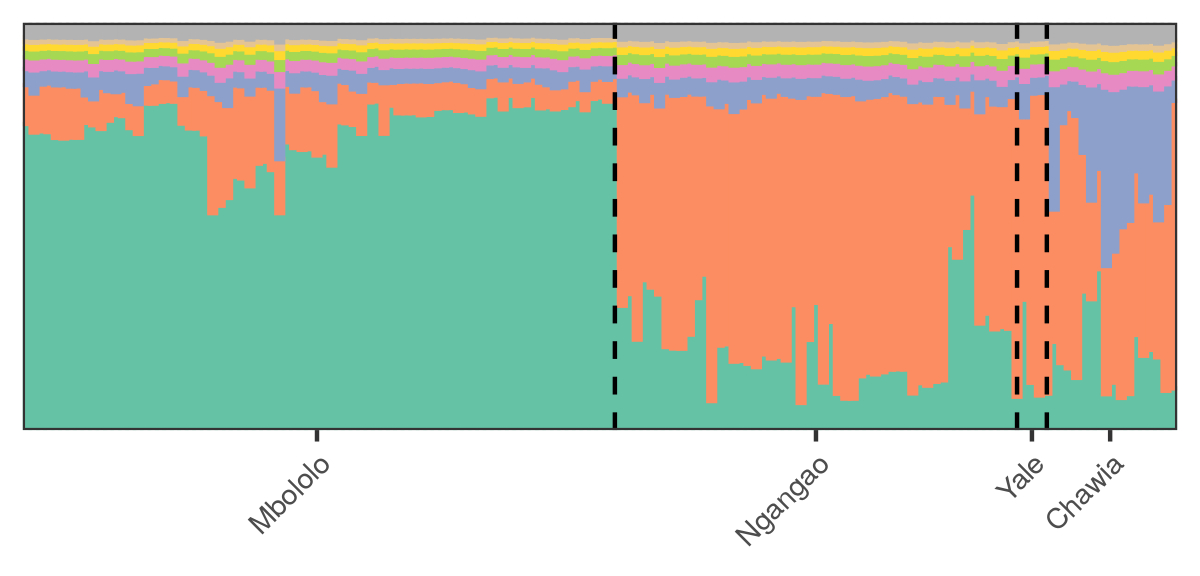
\includegraphics[width = 0.9\textwidth]{./figure/structure_init-1.png}
\caption*{The intitial fit at $\alpha = 3$. }
\end{figure}
\end{frame}


\begin{frame}{fastSTRUCTURE: Parametric Sensitivity}
  \begin{figure}[!h]
    \centering
    \only<1>{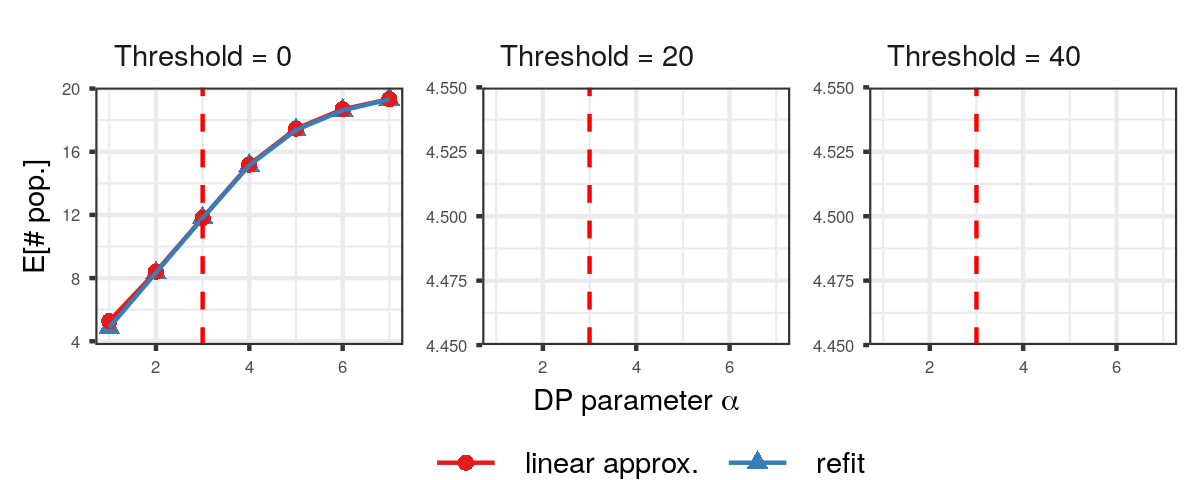
\includegraphics[width = \textwidth]{./figure/structure_alphasens0-1.png}}%
    \only<2>{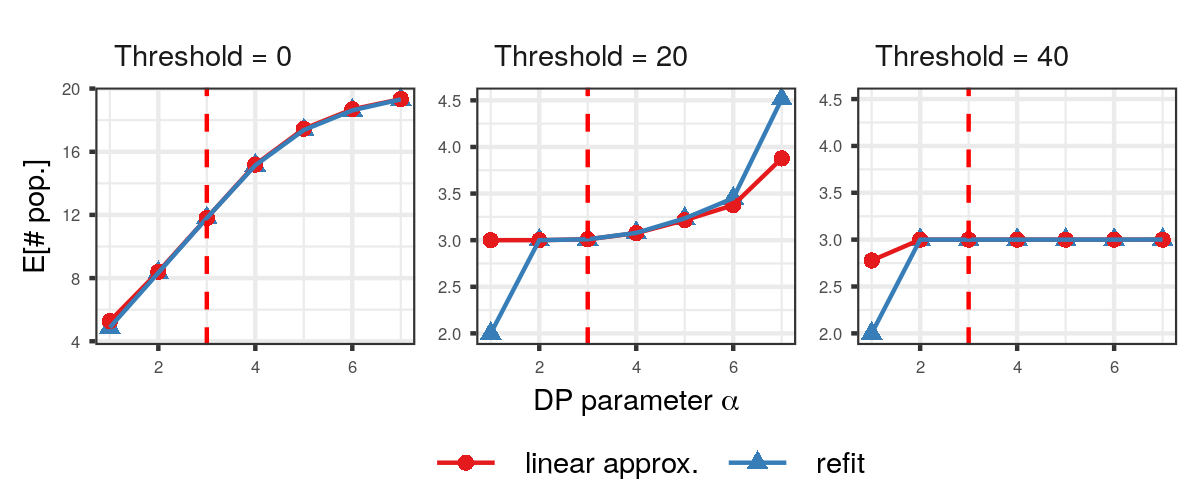
\includegraphics[width = \textwidth]{./figure/structure_alphasens-1.png}}
    \caption*{Expected number of posterior in-sample clusters in the thrush data as $\alpha$ varies.}
  \end{figure}

\end{frame}

\begin{frame}{fastSTRUCTURE: Evidence of Migration?}

  \begin{figure}[!h]
    \centering
    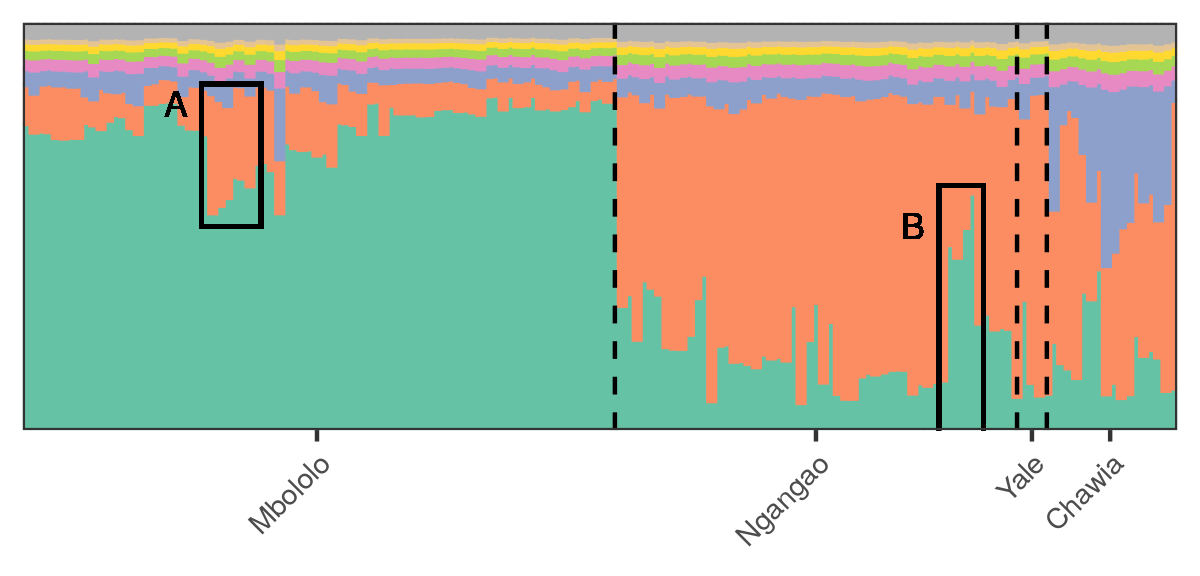
\includegraphics[width = 0.9\textwidth]{./figure/structure_migration-1.png}
  \end{figure}
\end{frame}

\begin{frame}{fastSTRUCTURE: Evidence of Migration?}
    \begin{figure}[!h]
\centering
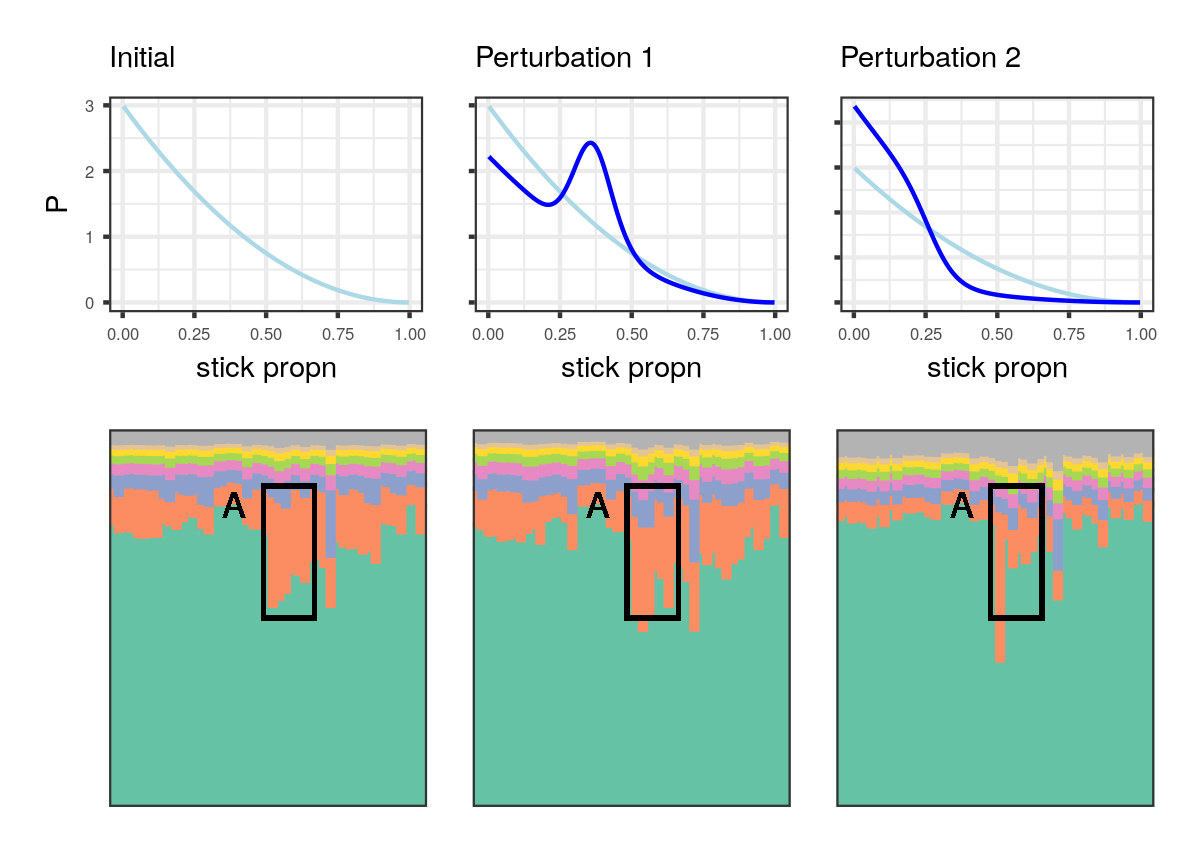
\includegraphics[width = \textwidth]{./figure/mbololo_motivating_ex-1.png}
\end{figure}

\end{frame}

\begin{frame}{fastSTRUCTURE: Functional Sensitivity}

\begin{figure}[!h]
    \centering
    \only<1>{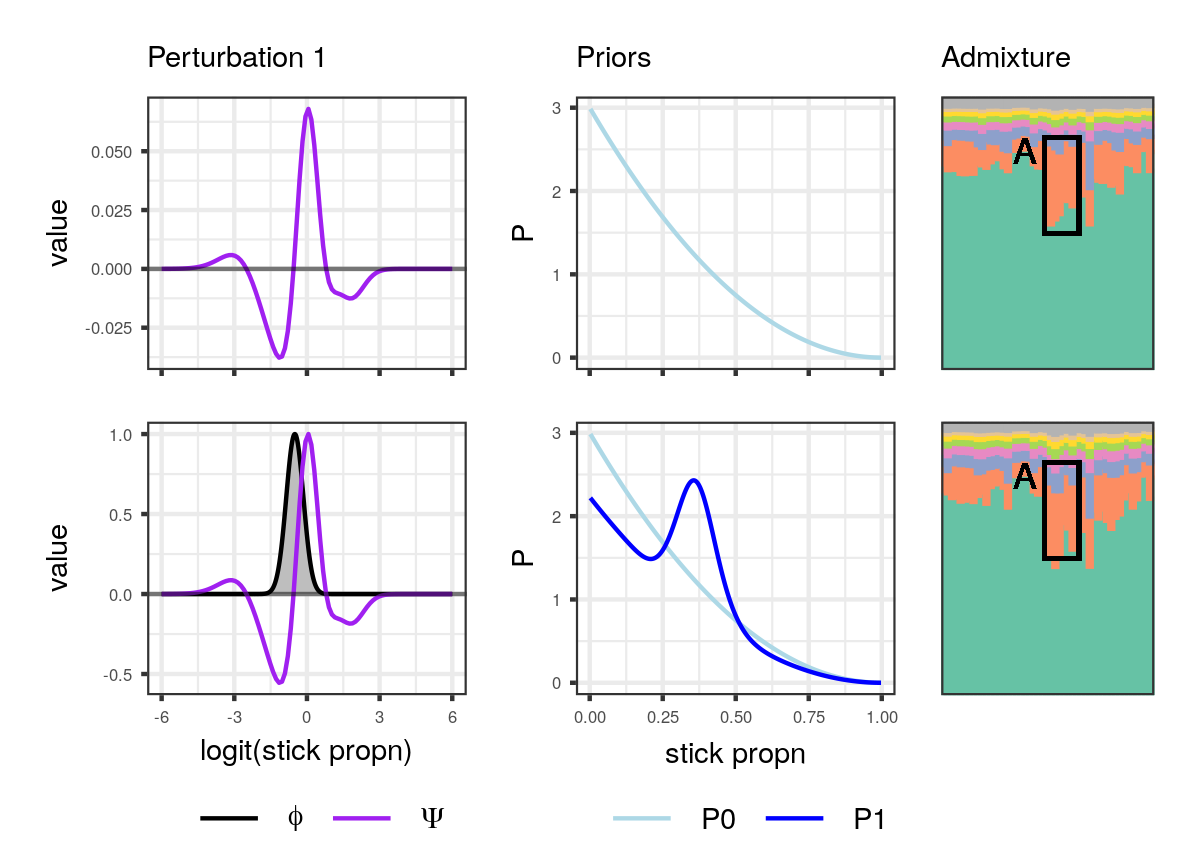
\includegraphics[width = \textwidth]{./figure/mbololo_motivating_ex_inflA-1.png}}
    \only<2>{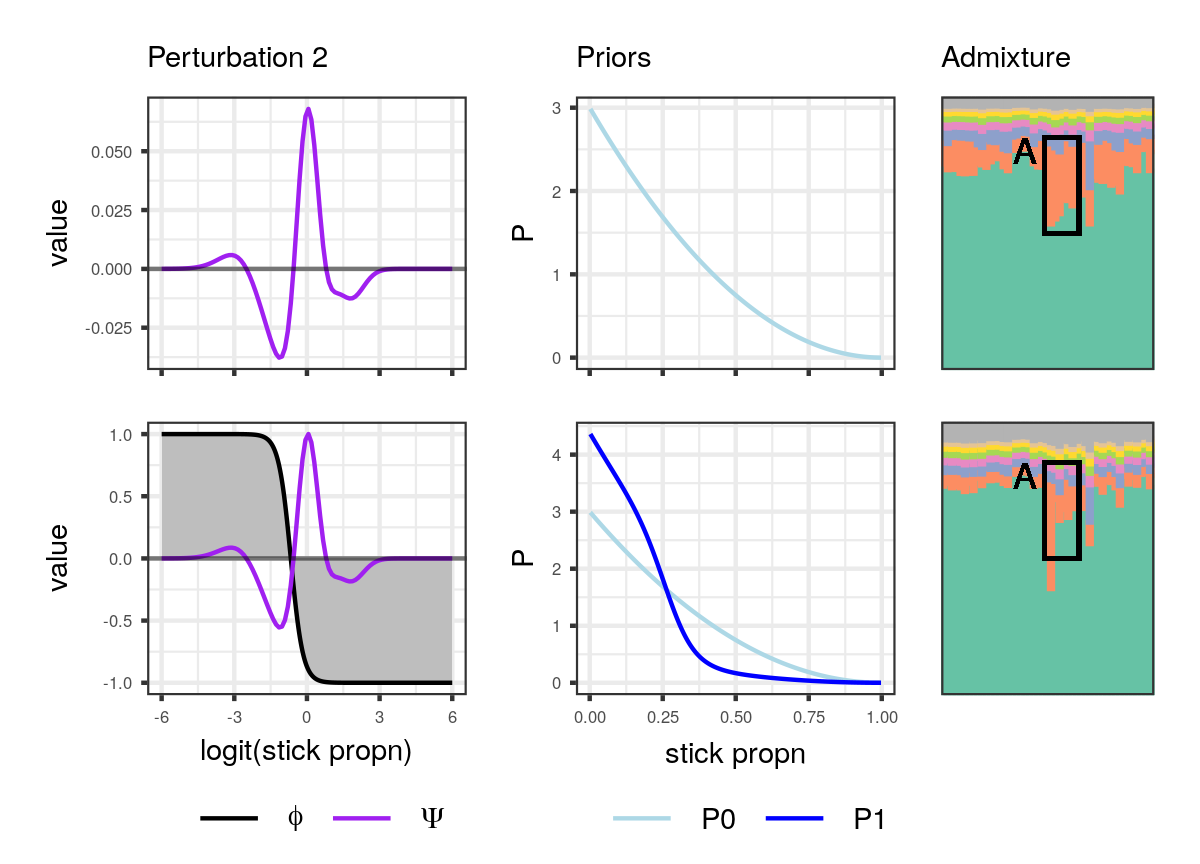
\includegraphics[width = \textwidth]{./figure/mbololo_motivating_ex_inflB-1.png}}
\end{figure}

\end{frame}

\begin{frame}{fastSTRUCTURE: Functional Sensitivity}

  \begin{figure}[!h]
    \centering
    \only<1>{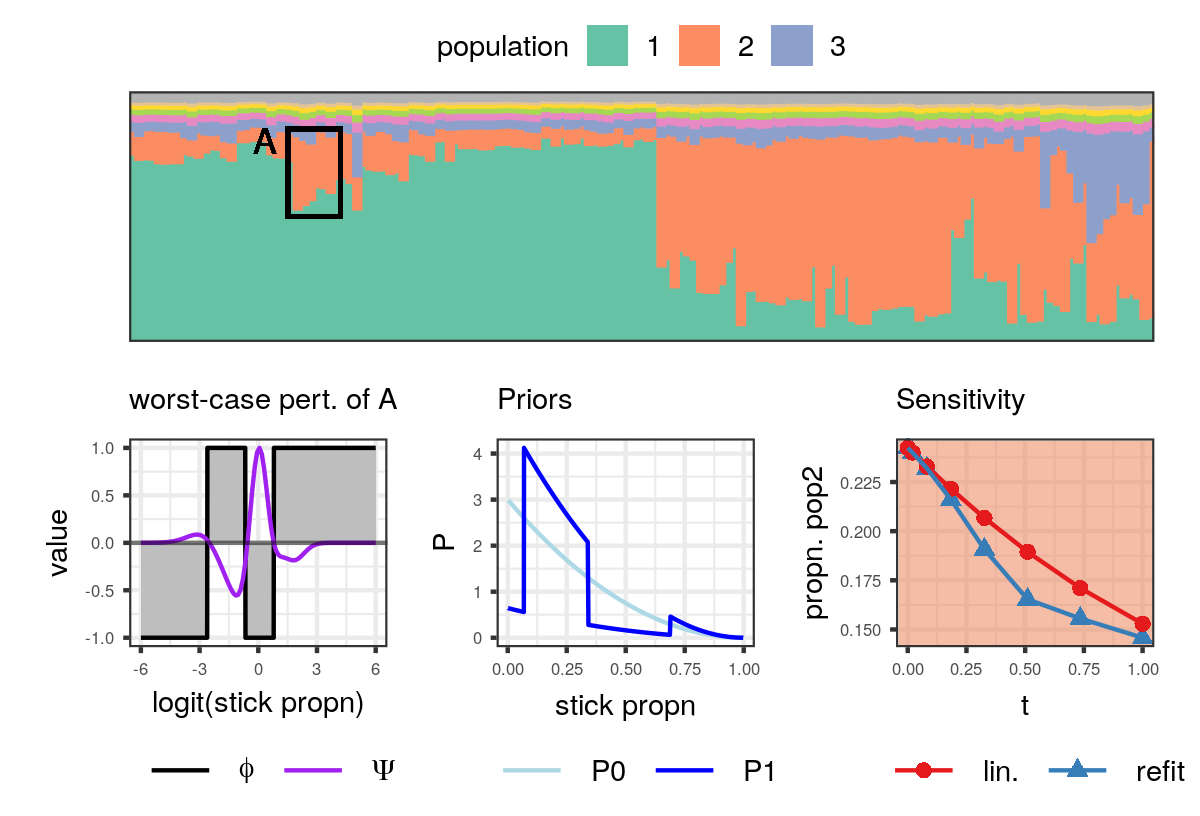
\includegraphics[width = \textwidth]{./figure/mbololo_outliers-1.png}}%
    \only<2>{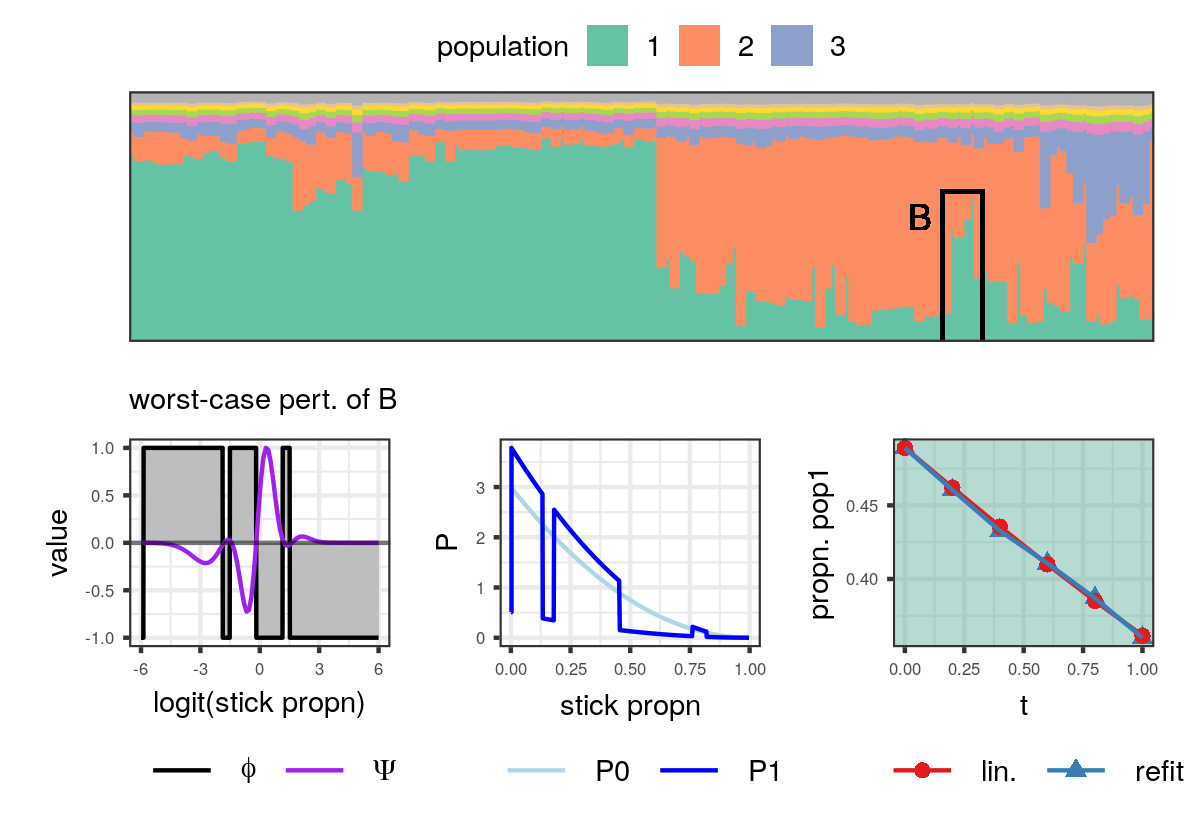
\includegraphics[width = \textwidth]{./figure/ngangao_outliers-1.png}}%
    % \only<3>{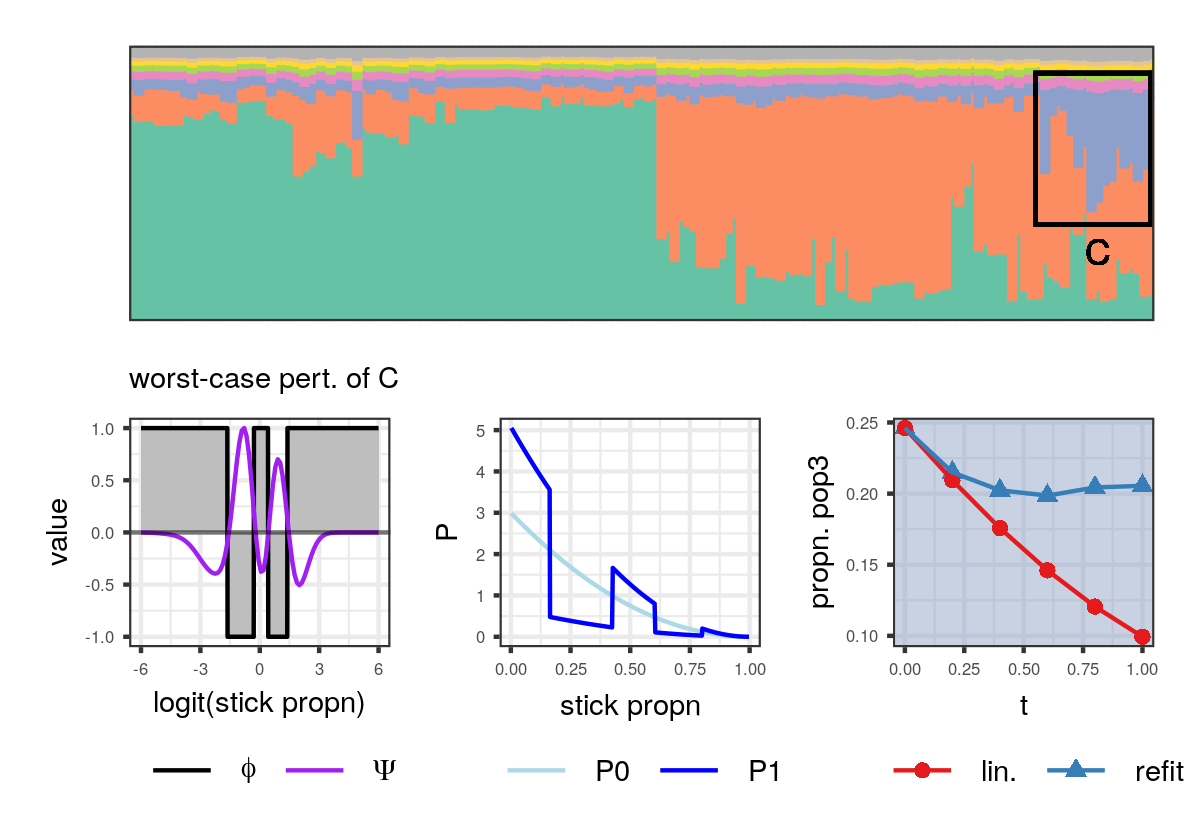
\includegraphics[width = \textwidth]{./figure/chawia_outliers-1.png}}
  \end{figure}

\end{frame}

%%%%%%%%%%%%%%%%%%%
% limitations of local sensitivity
%%%%%%%%%%%%%%%%%%%


\begin{frame}{Limitations of Local Sensitivity}
  \begin{figure}[!h]
    \centering
    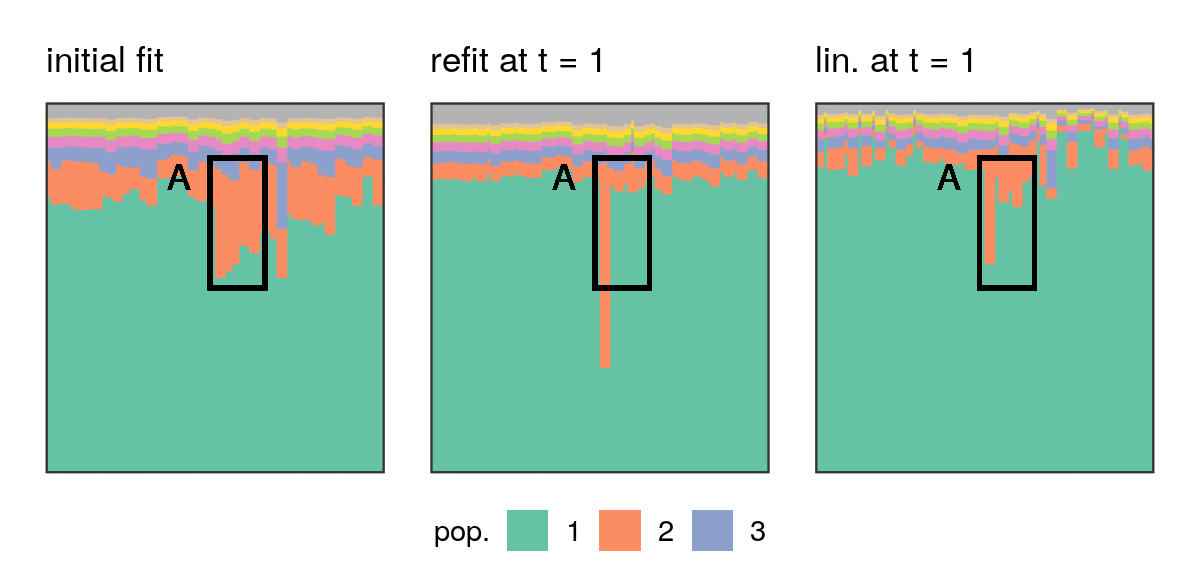
\includegraphics[width = \textwidth]{./figure/bad_admix_ex-1.png}
    \caption*{Inferred admixtures after the worst-case perturbation
     to individuals A.
     Individual $n = 26$ had a large increase in admixture proportion of
     population 2 after the refit. }
  \end{figure}

\end{frame}

\begin{frame}{Limitations of Local Sensitivity}

  \begin{figure}[!h]
    \centering
    \only<1>{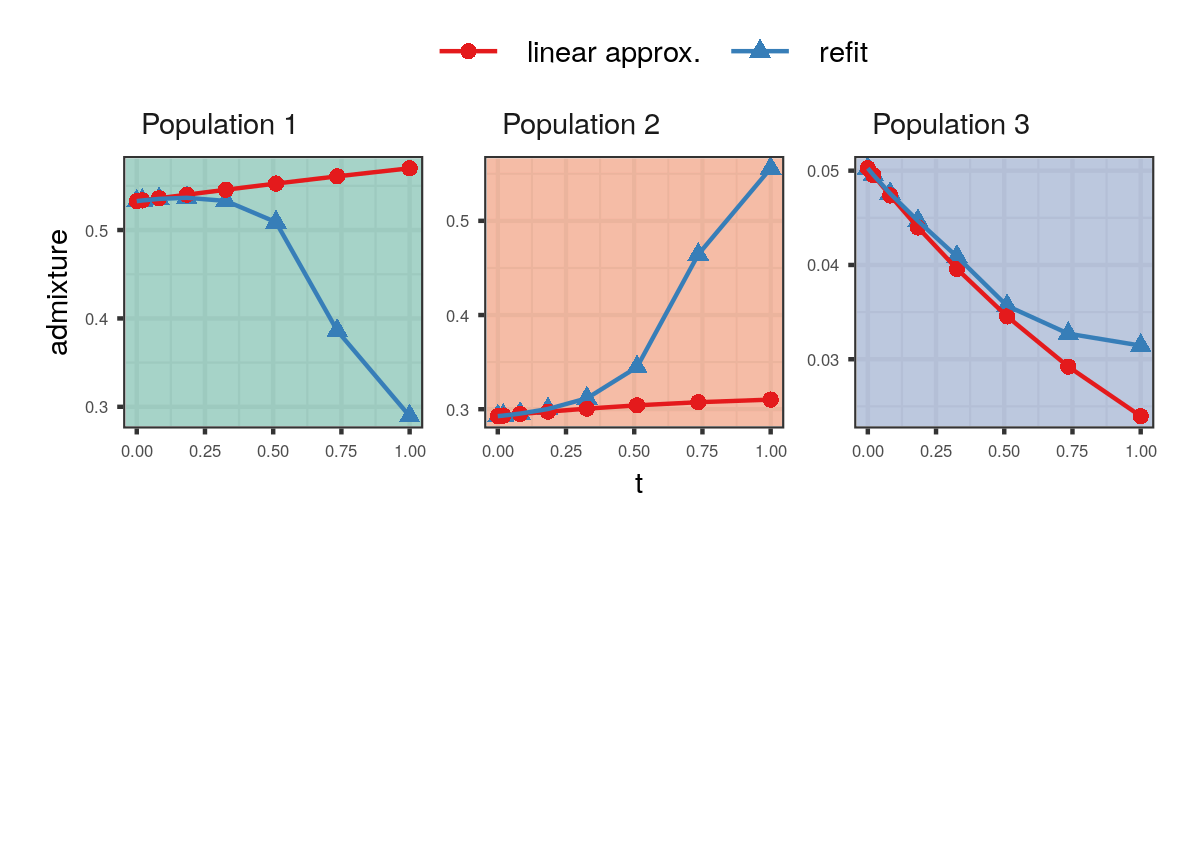
\includegraphics[width = \textwidth]{./figure/bad_admix_trace_admix-1.png}}%
    \only<2>{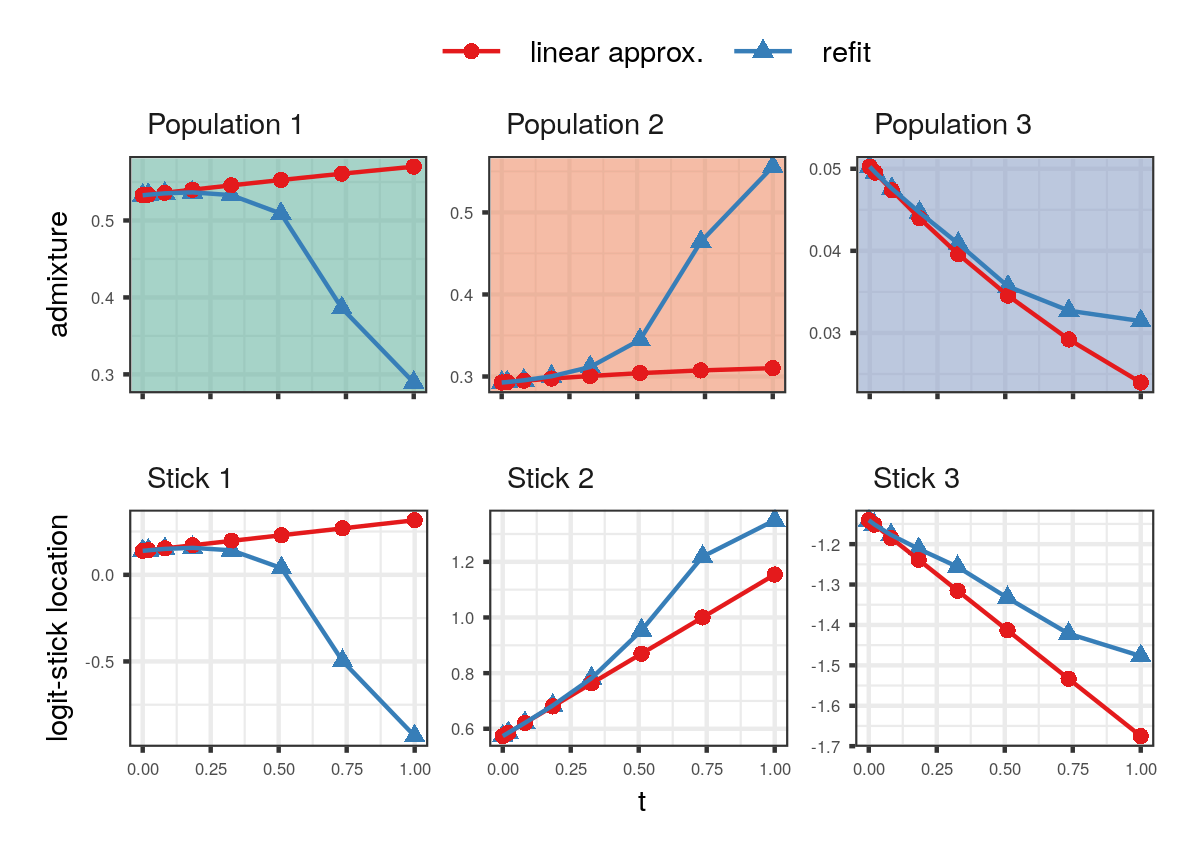
\includegraphics[width = \textwidth]{./figure/bad_admix_trace_all-1.png}}%
  \end{figure}

\end{frame}

\begin{frame}{Computational Complexity}

\begin{table}[tb]
\centering
\caption*{Compute time of results on the Taita thrush dataset. }
\begin{tabular}{|r|r|}
\hline
    & time (seconds) \\
    \hline
    Initial fit & 7 \\
    \hline
    Hessian solve for $\alpha$ sensitivity & 0.3\\
    Linear approx. $\eta^{lin}(\alpha)$ for $\alpha = 1, ..., 7$ &
        0.006 \\
    Refits $\eta(\alpha)$ for $\alpha = 1, ..., 7$ &
        30 \\
    \hline
    The influence function & 0.6 \\
    Hessian solve for perturbation $\phi$ &
        0.4 \\
    Linear approx. $\eta^{lin}(\epsilon)|_{\epsilon = 1}$
      for perturbation $\phi$ &
        0.001\\
    Refit $\eta(\epsilon)|_{\epsilon = 1}$
      for perturbation $\phi$ &
        10 \\
    \hline
\end{tabular}
\end{table}



\end{frame}


\begin{frame}{Conclusions}

\begin{itemize}
\item We provide a tool to efficiently evaluate the sensitivity of the variational posterior to prior choices.
\item Linearizing the variational parameters provides a reasonable alternative to
re-optimizing the variational approximation
after model perturbations.
\item For variational approximations based on KL divergence, one should express
functional perturbations multiplicatively.
\item The influence function can provide guidance for finding particularly sensitive model perturbations which can be investigated by re-fitting.
\end{itemize}

\end{frame}


\begin{frame}{Links and references}

\footnotesize

% {\bf A workshop paper: }\newline
Runjing Liu, Ryan Giordano, Michael I. Jordan, Tamara Broderick. \newline
“Evaluating Sensitivity to the Stick Breaking Prior in Bayesian Nonparametrics.”
\newline {\color{blue}\url{https://arxiv.org/pdf/1810.06587.pdf}}

% \vspace{0.5em}

% {\bf Code: }\newline
% Paragami: parameter folding and flattening for optimization problems \newline
% {\color{blue}\url{https://github.com/rgiordan/paragami}}
%
% Vittles: library for sensitivity analysis in optimization problems \newline
% {\color{blue}\url{https://pypi.org/project/vittles/}}
%
JAX: composable transformations of Python+NumPy programs \newline
{\color{blue}\url{https://github.com/google/jax}}
\vspace{-0.5em}

\par\noindent\rule{\textwidth}{0.4pt}

\vspace{-0.5em}

\bibliographystyle{plainnat}
% Hide the references header
% https://tex.stackexchange.com/questions/22645/hiding-the-title-of-the-bibliography/370784
\begingroup
\renewcommand{\section}[2]{}%
\bibliography{references}
\endgroup

\end{frame}



\end{document}
